% **************************************************************************************************************
% A Classic Thesis Style
% An Homage to The Elements of Typographic Style
%
% Copyright (C) 2012 Andr\'e Miede http://www.miede.de
%
% If you like the style then I would appreciate a postcard. My address 
% can be found in the file ClassicThesis.pdf. A collection of the 
% postcards I received so far is available online at 
% http://postcards.miede.de
%
% License:
% This program is free software; you can redistribute it and/or modify
% it under the terms of the GNU General Public License as published by
% the Free Software Foundation; either version 2 of the License, or
% (at your option) any later version.
%
% This program is distributed in the hope that it will be useful,
% but WITHOUT ANY WARRANTY; without even the implied warranty of
% MERCHANTABILITY or FITNESS FOR A PARTICULAR PURPOSE.  See the
% GNU General Public License for more details.
%
% You should have received a copy of the GNU General Public License
% along with this program; see the file COPYING.  If not, write to
% the Free Software Foundation, Inc., 59 Temple Place - Suite 330,
% Boston, MA 02111-1307, USA.
%
% **************************************************************************************************************
% Note:
%    * You must not use "u etc. in strings/commands that will be spaced out (use \"u or real umlauts instead)
%    * New enumeration (small caps): \begin{aenumerate} \end{aenumerate}
%    * For margin notes: \marginpar or \graffito{}
%    * Do not use bold fonts in this style, it is designed around them
%    * Use tables as in the examples
%    * See classicthesis-preamble.sty for useful commands
% **************************************************************************************************************
% To Do:
%		 * [high] Check this out: http://www.golatex.de/koma-script-warnung-in-verbindung-mit-listings-package-t2058.html
%    * [medium] mathbb in section-titles/chapter-titles => disappears somehow in headlines!!!
% **************************************************************************************************************
\documentclass[ twoside,openright,titlepage,numbers=noenddot,headinclude,%1headlines,% letterpaper a4paper
                footinclude=true,cleardoublepage=empty,abstractoff, % <--- obsolete, remove (todo)
                BCOR=5mm,paper=a4,fontsize=11pt,%11pt,a4paper,%
                ngerman,american,%
                ]{scrreprt}

%********************************************************************
% Note: Make all your adjustments in here
%*******************************************************
% ****************************************************************************************************
% classicthesis-config.tex 
% formerly known as loadpackages.sty, classicthesis-ldpkg.sty, and classicthesis-preamble.sty 
% Use it at the beginning of your ClassicThesis.tex, or as a LaTeX Preamble 
% in your ClassicThesis.{tex,lyx} with % ****************************************************************************************************
% classicthesis-config.tex 
% formerly known as loadpackages.sty, classicthesis-ldpkg.sty, and classicthesis-preamble.sty 
% Use it at the beginning of your ClassicThesis.tex, or as a LaTeX Preamble 
% in your ClassicThesis.{tex,lyx} with % ****************************************************************************************************
% classicthesis-config.tex 
% formerly known as loadpackages.sty, classicthesis-ldpkg.sty, and classicthesis-preamble.sty 
% Use it at the beginning of your ClassicThesis.tex, or as a LaTeX Preamble 
% in your ClassicThesis.{tex,lyx} with \input{classicthesis-config}
% ****************************************************************************************************  
% If you like the classicthesis, then I would appreciate a postcard. 
% My address can be found in the file ClassicThesis.pdf. A collection 
% of the postcards I received so far is available online at 
% http://postcards.miede.de
% ****************************************************************************************************

% ****************************************************************************************************
% 1. Configure classicthesis for your needs here, e.g., remove "drafting" below 
% in order to deactivate the time-stamp on the pages
% ****************************************************************************************************
\PassOptionsToPackage{eulerchapternumbers,listings,%
				 pdfspacing,%floatperchapter,%linedheaders,%
				 subfig,beramono,eulermath,parts}{classicthesis}										
% ********************************************************************
% Available options for classicthesis.sty 
% (see ClassicThesis.pdf for more information):
% drafting
% parts nochapters linedheaders
% eulerchapternumbers beramono eulermath pdfspacing minionprospacing
% tocaligned dottedtoc manychapters
% listings floatperchapter subfig
% ********************************************************************

% ********************************************************************
% Triggers for this config
% ******************************************************************** 
\usepackage{ifthen}
\newboolean{enable-backrefs} % enable backrefs in the bibliography
\setboolean{enable-backrefs}{false} % true false
% ****************************************************************************************************


% ****************************************************************************************************
% 2. Personal data and user ad-hoc commands
% ****************************************************************************************************
\newcommand{\myTitle}{Spatial analysis of complex biological tissues from single cell gene expression data\xspace}
\newcommand{\mySubtitle}{Clustering and visualizing functional tissues in \platy\xspace}
\newcommand{\myDegree}{Degree of Doctor of Philosophy (PhD)\xspace}
\newcommand{\myName}{Jean-Baptiste Olivier Georges Pettit\xspace}
\newcommand{\myProf}{Put name here\xspace}
\newcommand{\myOtherProf}{Put name here\xspace}
\newcommand{\mySupervisor}{Dr. John C. Marioni\xspace}
\newcommand{\myFaculty}{Put data here\xspace}
\newcommand{\myDepartment}{EMBL-EBI, European Molecular Biology Laboratory - European Bioinformatics Institute\xspace}
\newcommand{\myUni}{University of Cambridge\xspace}
\newcommand{\myLocation}{Cambridge\xspace}
\newcommand{\myTime}{2014\xspace}
\newcommand{\myVersion}{version 0.9\xspace}


% ********************************************************************
% Setup, finetuning, and useful commands
% ********************************************************************
\newcounter{dummy} % necessary for correct hyperlinks (to index, bib, etc.)
\newlength{\abcd} % for ab..z string length calculation
\providecommand{\mLyX}{L\kern-.1667em\lower.25em\hbox{Y}\kern-.125emX\@}
\newcommand{\ie}{i.\,e.}
\newcommand{\Ie}{I.\,e.}
\newcommand{\eg}{e.\,g.}
\newcommand{\Eg}{E.\,g.} 
% ****************************************************************************************************


% ****************************************************************************************************
% 3. Loading some handy packages
% ****************************************************************************************************
% ******************************************************************** 
% Packages with options that might require adjustments
% ******************************************************************** 
\PassOptionsToPackage{latin9}{inputenc}	% latin9 (ISO-8859-9) = latin1+"Euro sign"
 \usepackage{inputenc}				

%\PassOptionsToPackage{ngerman,american}{babel}   % change this to your language(s)
% Spanish languages need extra options in order to work with this template
%\PassOptionsToPackage{spanish,es-lcroman}{babel}
 \usepackage{babel}
					

\PassOptionsToPackage{square,numbers}{natbib}
 \usepackage{natbib}				

%\PassOptionsToPackage{fleqn}{amsmath}		% math environments and more by the AMS 
 \usepackage{amsmath}

% ******************************************************************** 
% General useful packages
% ******************************************************************** 
\PassOptionsToPackage{T1}{fontenc} % T2A for cyrillics
	\usepackage{fontenc}     
\usepackage{textcomp} % fix warning with missing font shapes
%\usepackage{scrhack} % fix warnings when using KOMA with listings package          
\usepackage{xspace} % to get the spacing after macros right  
\usepackage{mparhack} % get marginpar right
\usepackage{fixltx2e} % fixes some LaTeX stuff 
\PassOptionsToPackage{printonlyused,smaller}{acronym}
	\usepackage{acronym} % nice macros for handling all acronyms in the thesis
%\renewcommand*{\acsfont}[1]{\textssc{#1}} % for MinionPro
\renewcommand{\bflabel}[1]{{#1}\hfill} % fix the list of acronyms
% ****************************************************************************************************


% ****************************************************************************************************
% 4. Setup floats: tables, (sub)figures, and captions
% ****************************************************************************************************
\usepackage{tabularx} % better tables
	\setlength{\extrarowheight}{3pt} % increase table row height
\newcommand{\tableheadline}[1]{\multicolumn{1}{c}{\spacedlowsmallcaps{#1}}}
\newcommand{\myfloatalign}{\centering} % to be used with each float for alignment
\usepackage{caption}
\captionsetup{format=hang,font=small}
\usepackage{subfig}  
% ****************************************************************************************************


% ****************************************************************************************************
% 5. Setup code listings
% ****************************************************************************************************
\usepackage{listings} 
%\lstset{emph={trueIndex,root},emphstyle=\color{BlueViolet}}%\underbar} % for special keywords
\lstset{language=[LaTeX]Tex,%C++,
    keywordstyle=\color{RoyalBlue},%\bfseries,
    basicstyle=\small\ttfamily,
    %identifierstyle=\color{NavyBlue},
    commentstyle=\color{Green}\ttfamily,
    stringstyle=\rmfamily,
    numbers=none,%left,%
    numberstyle=\scriptsize,%\tiny
    stepnumber=5,
    numbersep=8pt,
    showstringspaces=false,
    breaklines=true,
    frameround=ftff,
    frame=single,
    belowcaptionskip=.75\baselineskip
    %frame=L
} 
% ****************************************************************************************************    		   


% ****************************************************************************************************
% 6. PDFLaTeX, hyperreferences and citation backreferences
% ****************************************************************************************************
% ********************************************************************
% Using PDFLaTeX
% ********************************************************************
\PassOptionsToPackage{pdftex,hyperfootnotes=false,pdfpagelabels}{hyperref}
	\usepackage{hyperref}  % backref linktocpage pagebackref
\pdfcompresslevel=9
\pdfadjustspacing=1 
\PassOptionsToPackage{pdftex}{graphicx}
	\usepackage{graphicx} 

% ********************************************************************
% Setup the style of the backrefs from the bibliography
% (translate the options to any language you use)
% ********************************************************************
\newcommand{\backrefnotcitedstring}{\relax}%(Not cited.)
\newcommand{\backrefcitedsinglestring}[1]{(Cited on page~#1.)}
\newcommand{\backrefcitedmultistring}[1]{(Cited on pages~#1.)}
\ifthenelse{\boolean{enable-backrefs}}%
{%
		\PassOptionsToPackage{hyperpageref}{backref}
		\usepackage{backref} % to be loaded after hyperref package 
		   \renewcommand{\backreftwosep}{ and~} % separate 2 pages
		   \renewcommand{\backreflastsep}{, and~} % separate last of longer list
		   \renewcommand*{\backref}[1]{}  % disable standard
		   \renewcommand*{\backrefalt}[4]{% detailed backref
		      \ifcase #1 %
		         \backrefnotcitedstring%
		      \or%
		         \backrefcitedsinglestring{#2}%
		      \else%
		         \backrefcitedmultistring{#2}%
		      \fi}%
}{\relax}    

% ********************************************************************
% Hyperreferences
% ********************************************************************
\hypersetup{%
    %draft,	% = no hyperlinking at all (useful in b/w printouts)
    colorlinks=true, linktocpage=true, pdfstartpage=3, pdfstartview=FitV,%
    % uncomment the following line if you want to have black links (e.g., for printing)
    %colorlinks=false, linktocpage=false, pdfborder={0 0 0}, pdfstartpage=3, pdfstartview=FitV,% 
    breaklinks=true, pdfpagemode=UseNone, pageanchor=true, pdfpagemode=UseOutlines,%
    plainpages=false, bookmarksnumbered, bookmarksopen=true, bookmarksopenlevel=1,%
    hypertexnames=true, pdfhighlight=/O,%nesting=true,%frenchlinks,%
    urlcolor=webbrown, linkcolor=RoyalBlue, citecolor=webgreen, %pagecolor=RoyalBlue,%
    %urlcolor=Black, linkcolor=Black, citecolor=Black, %pagecolor=Black,%
    pdftitle={\myTitle},%
    pdfauthor={\textcopyright\ \myName, \myUni, \myFaculty},%
    pdfsubject={},%
    pdfkeywords={},%
    pdfcreator={pdfLaTeX},%
    pdfproducer={LaTeX with hyperref and classicthesis}%
}   

% ********************************************************************
% Setup autoreferences
% ********************************************************************
% There are some issues regarding autorefnames
% http://www.ureader.de/msg/136221647.aspx
% http://www.tex.ac.uk/cgi-bin/texfaq2html?label=latexwords
% you have to redefine the makros for the 
% language you use, e.g., american, ngerman
% (as chosen when loading babel/AtBeginDocument)
% ********************************************************************
\makeatletter
\@ifpackageloaded{babel}%
    {%
       \addto\extrasamerican{%
					\renewcommand*{\figureautorefname}{Figure}%
					\renewcommand*{\tableautorefname}{Table}%
					\renewcommand*{\partautorefname}{Part}%
					\renewcommand*{\chapterautorefname}{Chapter}%
					\renewcommand*{\sectionautorefname}{Section}%
					\renewcommand*{\subsectionautorefname}{Section}%
					\renewcommand*{\subsubsectionautorefname}{Section}% 	
				}%
       \addto\extrasngerman{% 
					\renewcommand*{\paragraphautorefname}{Absatz}%
					\renewcommand*{\subparagraphautorefname}{Unterabsatz}%
					\renewcommand*{\footnoteautorefname}{Fu\"snote}%
					\renewcommand*{\FancyVerbLineautorefname}{Zeile}%
					\renewcommand*{\theoremautorefname}{Theorem}%
					\renewcommand*{\appendixautorefname}{Anhang}%
					\renewcommand*{\equationautorefname}{Gleichung}%        
					\renewcommand*{\itemautorefname}{Punkt}%
				}%	
			% Fix to getting autorefs for subfigures right (thanks to Belinda Vogt for changing the definition)
			\providecommand{\subfigureautorefname}{\figureautorefname}%  			
    }{\relax}
\makeatother


% ****************************************************************************************************
% 7. Last calls before the bar closes
% ****************************************************************************************************
% ********************************************************************
% Development Stuff
% ********************************************************************
\listfiles
%\PassOptionsToPackage{l2tabu,orthodox,abort}{nag}
%	\usepackage{nag}
%\PassOptionsToPackage{warning, all}{onlyamsmath}
%	\usepackage{onlyamsmath}

% ********************************************************************
% Last, but not least...
% ********************************************************************
\usepackage{classicthesis} 
% ****************************************************************************************************


% ****************************************************************************************************
% 8. Further adjustments (experimental)
% ****************************************************************************************************
% ********************************************************************
% Changing the text area
% ********************************************************************
%\linespread{1.05} % a bit more for Palatino
%\areaset[current]{312pt}{761pt} % 686 (factor 2.2) + 33 head + 42 head \the\footskip
%\setlength{\marginparwidth}{7em}%
%\setlength{\marginparsep}{2em}%

% ********************************************************************
% Using different fonts
% ********************************************************************
%\usepackage[oldstylenums]{kpfonts} % oldstyle notextcomp
%\usepackage[osf]{libertine}
%\usepackage{hfoldsty} % Computer Modern with osf
%\usepackage[light,condensed,math]{iwona}
%\renewcommand{\sfdefault}{iwona}
%\usepackage{lmodern} % <-- no osf support :-(
%\usepackage[urw-garamond]{mathdesign} <-- no osf support :-(
% ****************************************************************************************************

% ****************************************************************************************************  
% If you like the classicthesis, then I would appreciate a postcard. 
% My address can be found in the file ClassicThesis.pdf. A collection 
% of the postcards I received so far is available online at 
% http://postcards.miede.de
% ****************************************************************************************************

% ****************************************************************************************************
% 1. Configure classicthesis for your needs here, e.g., remove "drafting" below 
% in order to deactivate the time-stamp on the pages
% ****************************************************************************************************
\PassOptionsToPackage{eulerchapternumbers,listings,%
				 pdfspacing,%floatperchapter,%linedheaders,%
				 subfig,beramono,eulermath,parts}{classicthesis}										
% ********************************************************************
% Available options for classicthesis.sty 
% (see ClassicThesis.pdf for more information):
% drafting
% parts nochapters linedheaders
% eulerchapternumbers beramono eulermath pdfspacing minionprospacing
% tocaligned dottedtoc manychapters
% listings floatperchapter subfig
% ********************************************************************

% ********************************************************************
% Triggers for this config
% ******************************************************************** 
\usepackage{ifthen}
\newboolean{enable-backrefs} % enable backrefs in the bibliography
\setboolean{enable-backrefs}{false} % true false
% ****************************************************************************************************


% ****************************************************************************************************
% 2. Personal data and user ad-hoc commands
% ****************************************************************************************************
\newcommand{\myTitle}{Spatial analysis of complex biological tissues from single cell gene expression data\xspace}
\newcommand{\mySubtitle}{Clustering and visualizing functional tissues in \platy\xspace}
\newcommand{\myDegree}{Degree of Doctor of Philosophy (PhD)\xspace}
\newcommand{\myName}{Jean-Baptiste Olivier Georges Pettit\xspace}
\newcommand{\myProf}{Put name here\xspace}
\newcommand{\myOtherProf}{Put name here\xspace}
\newcommand{\mySupervisor}{Dr. John C. Marioni\xspace}
\newcommand{\myFaculty}{Put data here\xspace}
\newcommand{\myDepartment}{EMBL-EBI, European Molecular Biology Laboratory - European Bioinformatics Institute\xspace}
\newcommand{\myUni}{University of Cambridge\xspace}
\newcommand{\myLocation}{Cambridge\xspace}
\newcommand{\myTime}{2014\xspace}
\newcommand{\myVersion}{version 0.9\xspace}


% ********************************************************************
% Setup, finetuning, and useful commands
% ********************************************************************
\newcounter{dummy} % necessary for correct hyperlinks (to index, bib, etc.)
\newlength{\abcd} % for ab..z string length calculation
\providecommand{\mLyX}{L\kern-.1667em\lower.25em\hbox{Y}\kern-.125emX\@}
\newcommand{\ie}{i.\,e.}
\newcommand{\Ie}{I.\,e.}
\newcommand{\eg}{e.\,g.}
\newcommand{\Eg}{E.\,g.} 
% ****************************************************************************************************


% ****************************************************************************************************
% 3. Loading some handy packages
% ****************************************************************************************************
% ******************************************************************** 
% Packages with options that might require adjustments
% ******************************************************************** 
\PassOptionsToPackage{latin9}{inputenc}	% latin9 (ISO-8859-9) = latin1+"Euro sign"
 \usepackage{inputenc}				

%\PassOptionsToPackage{ngerman,american}{babel}   % change this to your language(s)
% Spanish languages need extra options in order to work with this template
%\PassOptionsToPackage{spanish,es-lcroman}{babel}
 \usepackage{babel}
					

\PassOptionsToPackage{square,numbers}{natbib}
 \usepackage{natbib}				

%\PassOptionsToPackage{fleqn}{amsmath}		% math environments and more by the AMS 
 \usepackage{amsmath}

% ******************************************************************** 
% General useful packages
% ******************************************************************** 
\PassOptionsToPackage{T1}{fontenc} % T2A for cyrillics
	\usepackage{fontenc}     
\usepackage{textcomp} % fix warning with missing font shapes
%\usepackage{scrhack} % fix warnings when using KOMA with listings package          
\usepackage{xspace} % to get the spacing after macros right  
\usepackage{mparhack} % get marginpar right
\usepackage{fixltx2e} % fixes some LaTeX stuff 
\PassOptionsToPackage{printonlyused,smaller}{acronym}
	\usepackage{acronym} % nice macros for handling all acronyms in the thesis
%\renewcommand*{\acsfont}[1]{\textssc{#1}} % for MinionPro
\renewcommand{\bflabel}[1]{{#1}\hfill} % fix the list of acronyms
% ****************************************************************************************************


% ****************************************************************************************************
% 4. Setup floats: tables, (sub)figures, and captions
% ****************************************************************************************************
\usepackage{tabularx} % better tables
	\setlength{\extrarowheight}{3pt} % increase table row height
\newcommand{\tableheadline}[1]{\multicolumn{1}{c}{\spacedlowsmallcaps{#1}}}
\newcommand{\myfloatalign}{\centering} % to be used with each float for alignment
\usepackage{caption}
\captionsetup{format=hang,font=small}
\usepackage{subfig}  
% ****************************************************************************************************


% ****************************************************************************************************
% 5. Setup code listings
% ****************************************************************************************************
\usepackage{listings} 
%\lstset{emph={trueIndex,root},emphstyle=\color{BlueViolet}}%\underbar} % for special keywords
\lstset{language=[LaTeX]Tex,%C++,
    keywordstyle=\color{RoyalBlue},%\bfseries,
    basicstyle=\small\ttfamily,
    %identifierstyle=\color{NavyBlue},
    commentstyle=\color{Green}\ttfamily,
    stringstyle=\rmfamily,
    numbers=none,%left,%
    numberstyle=\scriptsize,%\tiny
    stepnumber=5,
    numbersep=8pt,
    showstringspaces=false,
    breaklines=true,
    frameround=ftff,
    frame=single,
    belowcaptionskip=.75\baselineskip
    %frame=L
} 
% ****************************************************************************************************    		   


% ****************************************************************************************************
% 6. PDFLaTeX, hyperreferences and citation backreferences
% ****************************************************************************************************
% ********************************************************************
% Using PDFLaTeX
% ********************************************************************
\PassOptionsToPackage{pdftex,hyperfootnotes=false,pdfpagelabels}{hyperref}
	\usepackage{hyperref}  % backref linktocpage pagebackref
\pdfcompresslevel=9
\pdfadjustspacing=1 
\PassOptionsToPackage{pdftex}{graphicx}
	\usepackage{graphicx} 

% ********************************************************************
% Setup the style of the backrefs from the bibliography
% (translate the options to any language you use)
% ********************************************************************
\newcommand{\backrefnotcitedstring}{\relax}%(Not cited.)
\newcommand{\backrefcitedsinglestring}[1]{(Cited on page~#1.)}
\newcommand{\backrefcitedmultistring}[1]{(Cited on pages~#1.)}
\ifthenelse{\boolean{enable-backrefs}}%
{%
		\PassOptionsToPackage{hyperpageref}{backref}
		\usepackage{backref} % to be loaded after hyperref package 
		   \renewcommand{\backreftwosep}{ and~} % separate 2 pages
		   \renewcommand{\backreflastsep}{, and~} % separate last of longer list
		   \renewcommand*{\backref}[1]{}  % disable standard
		   \renewcommand*{\backrefalt}[4]{% detailed backref
		      \ifcase #1 %
		         \backrefnotcitedstring%
		      \or%
		         \backrefcitedsinglestring{#2}%
		      \else%
		         \backrefcitedmultistring{#2}%
		      \fi}%
}{\relax}    

% ********************************************************************
% Hyperreferences
% ********************************************************************
\hypersetup{%
    %draft,	% = no hyperlinking at all (useful in b/w printouts)
    colorlinks=true, linktocpage=true, pdfstartpage=3, pdfstartview=FitV,%
    % uncomment the following line if you want to have black links (e.g., for printing)
    %colorlinks=false, linktocpage=false, pdfborder={0 0 0}, pdfstartpage=3, pdfstartview=FitV,% 
    breaklinks=true, pdfpagemode=UseNone, pageanchor=true, pdfpagemode=UseOutlines,%
    plainpages=false, bookmarksnumbered, bookmarksopen=true, bookmarksopenlevel=1,%
    hypertexnames=true, pdfhighlight=/O,%nesting=true,%frenchlinks,%
    urlcolor=webbrown, linkcolor=RoyalBlue, citecolor=webgreen, %pagecolor=RoyalBlue,%
    %urlcolor=Black, linkcolor=Black, citecolor=Black, %pagecolor=Black,%
    pdftitle={\myTitle},%
    pdfauthor={\textcopyright\ \myName, \myUni, \myFaculty},%
    pdfsubject={},%
    pdfkeywords={},%
    pdfcreator={pdfLaTeX},%
    pdfproducer={LaTeX with hyperref and classicthesis}%
}   

% ********************************************************************
% Setup autoreferences
% ********************************************************************
% There are some issues regarding autorefnames
% http://www.ureader.de/msg/136221647.aspx
% http://www.tex.ac.uk/cgi-bin/texfaq2html?label=latexwords
% you have to redefine the makros for the 
% language you use, e.g., american, ngerman
% (as chosen when loading babel/AtBeginDocument)
% ********************************************************************
\makeatletter
\@ifpackageloaded{babel}%
    {%
       \addto\extrasamerican{%
					\renewcommand*{\figureautorefname}{Figure}%
					\renewcommand*{\tableautorefname}{Table}%
					\renewcommand*{\partautorefname}{Part}%
					\renewcommand*{\chapterautorefname}{Chapter}%
					\renewcommand*{\sectionautorefname}{Section}%
					\renewcommand*{\subsectionautorefname}{Section}%
					\renewcommand*{\subsubsectionautorefname}{Section}% 	
				}%
       \addto\extrasngerman{% 
					\renewcommand*{\paragraphautorefname}{Absatz}%
					\renewcommand*{\subparagraphautorefname}{Unterabsatz}%
					\renewcommand*{\footnoteautorefname}{Fu\"snote}%
					\renewcommand*{\FancyVerbLineautorefname}{Zeile}%
					\renewcommand*{\theoremautorefname}{Theorem}%
					\renewcommand*{\appendixautorefname}{Anhang}%
					\renewcommand*{\equationautorefname}{Gleichung}%        
					\renewcommand*{\itemautorefname}{Punkt}%
				}%	
			% Fix to getting autorefs for subfigures right (thanks to Belinda Vogt for changing the definition)
			\providecommand{\subfigureautorefname}{\figureautorefname}%  			
    }{\relax}
\makeatother


% ****************************************************************************************************
% 7. Last calls before the bar closes
% ****************************************************************************************************
% ********************************************************************
% Development Stuff
% ********************************************************************
\listfiles
%\PassOptionsToPackage{l2tabu,orthodox,abort}{nag}
%	\usepackage{nag}
%\PassOptionsToPackage{warning, all}{onlyamsmath}
%	\usepackage{onlyamsmath}

% ********************************************************************
% Last, but not least...
% ********************************************************************
\usepackage{classicthesis} 
% ****************************************************************************************************


% ****************************************************************************************************
% 8. Further adjustments (experimental)
% ****************************************************************************************************
% ********************************************************************
% Changing the text area
% ********************************************************************
%\linespread{1.05} % a bit more for Palatino
%\areaset[current]{312pt}{761pt} % 686 (factor 2.2) + 33 head + 42 head \the\footskip
%\setlength{\marginparwidth}{7em}%
%\setlength{\marginparsep}{2em}%

% ********************************************************************
% Using different fonts
% ********************************************************************
%\usepackage[oldstylenums]{kpfonts} % oldstyle notextcomp
%\usepackage[osf]{libertine}
%\usepackage{hfoldsty} % Computer Modern with osf
%\usepackage[light,condensed,math]{iwona}
%\renewcommand{\sfdefault}{iwona}
%\usepackage{lmodern} % <-- no osf support :-(
%\usepackage[urw-garamond]{mathdesign} <-- no osf support :-(
% ****************************************************************************************************

% ****************************************************************************************************  
% If you like the classicthesis, then I would appreciate a postcard. 
% My address can be found in the file ClassicThesis.pdf. A collection 
% of the postcards I received so far is available online at 
% http://postcards.miede.de
% ****************************************************************************************************

% ****************************************************************************************************
% 1. Configure classicthesis for your needs here, e.g., remove "drafting" below 
% in order to deactivate the time-stamp on the pages
% ****************************************************************************************************
\PassOptionsToPackage{eulerchapternumbers,listings,%
				 pdfspacing,%floatperchapter,%linedheaders,%
				 subfig,beramono,eulermath,parts}{classicthesis}										
% ********************************************************************
% Available options for classicthesis.sty 
% (see ClassicThesis.pdf for more information):
% drafting
% parts nochapters linedheaders
% eulerchapternumbers beramono eulermath pdfspacing minionprospacing
% tocaligned dottedtoc manychapters
% listings floatperchapter subfig
% ********************************************************************

% ********************************************************************
% Triggers for this config
% ******************************************************************** 
\usepackage{ifthen}
\newboolean{enable-backrefs} % enable backrefs in the bibliography
\setboolean{enable-backrefs}{false} % true false
% ****************************************************************************************************


% ****************************************************************************************************
% 2. Personal data and user ad-hoc commands
% ****************************************************************************************************
\newcommand{\myTitle}{Spatial analysis of complex biological tissues from single cell gene expression data\xspace}
\newcommand{\mySubtitle}{Clustering and visualizing functional tissues in \platy\xspace}
\newcommand{\myDegree}{Degree of Doctor of Philosophy (PhD)\xspace}
\newcommand{\myName}{Jean-Baptiste Olivier Georges Pettit\xspace}
\newcommand{\myProf}{Put name here\xspace}
\newcommand{\myOtherProf}{Put name here\xspace}
\newcommand{\mySupervisor}{Dr. John C. Marioni\xspace}
\newcommand{\myFaculty}{Put data here\xspace}
\newcommand{\myDepartment}{EMBL-EBI, European Molecular Biology Laboratory - European Bioinformatics Institute\xspace}
\newcommand{\myUni}{University of Cambridge\xspace}
\newcommand{\myLocation}{Cambridge\xspace}
\newcommand{\myTime}{2014\xspace}
\newcommand{\myVersion}{version 0.9\xspace}


% ********************************************************************
% Setup, finetuning, and useful commands
% ********************************************************************
\newcounter{dummy} % necessary for correct hyperlinks (to index, bib, etc.)
\newlength{\abcd} % for ab..z string length calculation
\providecommand{\mLyX}{L\kern-.1667em\lower.25em\hbox{Y}\kern-.125emX\@}
\newcommand{\ie}{i.\,e.}
\newcommand{\Ie}{I.\,e.}
\newcommand{\eg}{e.\,g.}
\newcommand{\Eg}{E.\,g.} 
% ****************************************************************************************************


% ****************************************************************************************************
% 3. Loading some handy packages
% ****************************************************************************************************
% ******************************************************************** 
% Packages with options that might require adjustments
% ******************************************************************** 
\PassOptionsToPackage{latin9}{inputenc}	% latin9 (ISO-8859-9) = latin1+"Euro sign"
 \usepackage{inputenc}				

%\PassOptionsToPackage{ngerman,american}{babel}   % change this to your language(s)
% Spanish languages need extra options in order to work with this template
%\PassOptionsToPackage{spanish,es-lcroman}{babel}
 \usepackage{babel}
					

\PassOptionsToPackage{square,numbers}{natbib}
 \usepackage{natbib}				

%\PassOptionsToPackage{fleqn}{amsmath}		% math environments and more by the AMS 
 \usepackage{amsmath}

% ******************************************************************** 
% General useful packages
% ******************************************************************** 
\PassOptionsToPackage{T1}{fontenc} % T2A for cyrillics
	\usepackage{fontenc}     
\usepackage{textcomp} % fix warning with missing font shapes
%\usepackage{scrhack} % fix warnings when using KOMA with listings package          
\usepackage{xspace} % to get the spacing after macros right  
\usepackage{mparhack} % get marginpar right
\usepackage{fixltx2e} % fixes some LaTeX stuff 
\PassOptionsToPackage{printonlyused,smaller}{acronym}
	\usepackage{acronym} % nice macros for handling all acronyms in the thesis
%\renewcommand*{\acsfont}[1]{\textssc{#1}} % for MinionPro
\renewcommand{\bflabel}[1]{{#1}\hfill} % fix the list of acronyms
% ****************************************************************************************************


% ****************************************************************************************************
% 4. Setup floats: tables, (sub)figures, and captions
% ****************************************************************************************************
\usepackage{tabularx} % better tables
	\setlength{\extrarowheight}{3pt} % increase table row height
\newcommand{\tableheadline}[1]{\multicolumn{1}{c}{\spacedlowsmallcaps{#1}}}
\newcommand{\myfloatalign}{\centering} % to be used with each float for alignment
\usepackage{caption}
\captionsetup{format=hang,font=small}
\usepackage{subfig}  
% ****************************************************************************************************


% ****************************************************************************************************
% 5. Setup code listings
% ****************************************************************************************************
\usepackage{listings} 
%\lstset{emph={trueIndex,root},emphstyle=\color{BlueViolet}}%\underbar} % for special keywords
\lstset{language=[LaTeX]Tex,%C++,
    keywordstyle=\color{RoyalBlue},%\bfseries,
    basicstyle=\small\ttfamily,
    %identifierstyle=\color{NavyBlue},
    commentstyle=\color{Green}\ttfamily,
    stringstyle=\rmfamily,
    numbers=none,%left,%
    numberstyle=\scriptsize,%\tiny
    stepnumber=5,
    numbersep=8pt,
    showstringspaces=false,
    breaklines=true,
    frameround=ftff,
    frame=single,
    belowcaptionskip=.75\baselineskip
    %frame=L
} 
% ****************************************************************************************************    		   


% ****************************************************************************************************
% 6. PDFLaTeX, hyperreferences and citation backreferences
% ****************************************************************************************************
% ********************************************************************
% Using PDFLaTeX
% ********************************************************************
\PassOptionsToPackage{pdftex,hyperfootnotes=false,pdfpagelabels}{hyperref}
	\usepackage{hyperref}  % backref linktocpage pagebackref
\pdfcompresslevel=9
\pdfadjustspacing=1 
\PassOptionsToPackage{pdftex}{graphicx}
	\usepackage{graphicx} 

% ********************************************************************
% Setup the style of the backrefs from the bibliography
% (translate the options to any language you use)
% ********************************************************************
\newcommand{\backrefnotcitedstring}{\relax}%(Not cited.)
\newcommand{\backrefcitedsinglestring}[1]{(Cited on page~#1.)}
\newcommand{\backrefcitedmultistring}[1]{(Cited on pages~#1.)}
\ifthenelse{\boolean{enable-backrefs}}%
{%
		\PassOptionsToPackage{hyperpageref}{backref}
		\usepackage{backref} % to be loaded after hyperref package 
		   \renewcommand{\backreftwosep}{ and~} % separate 2 pages
		   \renewcommand{\backreflastsep}{, and~} % separate last of longer list
		   \renewcommand*{\backref}[1]{}  % disable standard
		   \renewcommand*{\backrefalt}[4]{% detailed backref
		      \ifcase #1 %
		         \backrefnotcitedstring%
		      \or%
		         \backrefcitedsinglestring{#2}%
		      \else%
		         \backrefcitedmultistring{#2}%
		      \fi}%
}{\relax}    

% ********************************************************************
% Hyperreferences
% ********************************************************************
\hypersetup{%
    %draft,	% = no hyperlinking at all (useful in b/w printouts)
    colorlinks=true, linktocpage=true, pdfstartpage=3, pdfstartview=FitV,%
    % uncomment the following line if you want to have black links (e.g., for printing)
    %colorlinks=false, linktocpage=false, pdfborder={0 0 0}, pdfstartpage=3, pdfstartview=FitV,% 
    breaklinks=true, pdfpagemode=UseNone, pageanchor=true, pdfpagemode=UseOutlines,%
    plainpages=false, bookmarksnumbered, bookmarksopen=true, bookmarksopenlevel=1,%
    hypertexnames=true, pdfhighlight=/O,%nesting=true,%frenchlinks,%
    urlcolor=webbrown, linkcolor=RoyalBlue, citecolor=webgreen, %pagecolor=RoyalBlue,%
    %urlcolor=Black, linkcolor=Black, citecolor=Black, %pagecolor=Black,%
    pdftitle={\myTitle},%
    pdfauthor={\textcopyright\ \myName, \myUni, \myFaculty},%
    pdfsubject={},%
    pdfkeywords={},%
    pdfcreator={pdfLaTeX},%
    pdfproducer={LaTeX with hyperref and classicthesis}%
}   

% ********************************************************************
% Setup autoreferences
% ********************************************************************
% There are some issues regarding autorefnames
% http://www.ureader.de/msg/136221647.aspx
% http://www.tex.ac.uk/cgi-bin/texfaq2html?label=latexwords
% you have to redefine the makros for the 
% language you use, e.g., american, ngerman
% (as chosen when loading babel/AtBeginDocument)
% ********************************************************************
\makeatletter
\@ifpackageloaded{babel}%
    {%
       \addto\extrasamerican{%
					\renewcommand*{\figureautorefname}{Figure}%
					\renewcommand*{\tableautorefname}{Table}%
					\renewcommand*{\partautorefname}{Part}%
					\renewcommand*{\chapterautorefname}{Chapter}%
					\renewcommand*{\sectionautorefname}{Section}%
					\renewcommand*{\subsectionautorefname}{Section}%
					\renewcommand*{\subsubsectionautorefname}{Section}% 	
				}%
       \addto\extrasngerman{% 
					\renewcommand*{\paragraphautorefname}{Absatz}%
					\renewcommand*{\subparagraphautorefname}{Unterabsatz}%
					\renewcommand*{\footnoteautorefname}{Fu\"snote}%
					\renewcommand*{\FancyVerbLineautorefname}{Zeile}%
					\renewcommand*{\theoremautorefname}{Theorem}%
					\renewcommand*{\appendixautorefname}{Anhang}%
					\renewcommand*{\equationautorefname}{Gleichung}%        
					\renewcommand*{\itemautorefname}{Punkt}%
				}%	
			% Fix to getting autorefs for subfigures right (thanks to Belinda Vogt for changing the definition)
			\providecommand{\subfigureautorefname}{\figureautorefname}%  			
    }{\relax}
\makeatother


% ****************************************************************************************************
% 7. Last calls before the bar closes
% ****************************************************************************************************
% ********************************************************************
% Development Stuff
% ********************************************************************
\listfiles
%\PassOptionsToPackage{l2tabu,orthodox,abort}{nag}
%	\usepackage{nag}
%\PassOptionsToPackage{warning, all}{onlyamsmath}
%	\usepackage{onlyamsmath}

% ********************************************************************
% Last, but not least...
% ********************************************************************
\usepackage{classicthesis} 
% ****************************************************************************************************


% ****************************************************************************************************
% 8. Further adjustments (experimental)
% ****************************************************************************************************
% ********************************************************************
% Changing the text area
% ********************************************************************
%\linespread{1.05} % a bit more for Palatino
%\areaset[current]{312pt}{761pt} % 686 (factor 2.2) + 33 head + 42 head \the\footskip
%\setlength{\marginparwidth}{7em}%
%\setlength{\marginparsep}{2em}%

% ********************************************************************
% Using different fonts
% ********************************************************************
%\usepackage[oldstylenums]{kpfonts} % oldstyle notextcomp
%\usepackage[osf]{libertine}
%\usepackage{hfoldsty} % Computer Modern with osf
%\usepackage[light,condensed,math]{iwona}
%\renewcommand{\sfdefault}{iwona}
%\usepackage{lmodern} % <-- no osf support :-(
%\usepackage[urw-garamond]{mathdesign} <-- no osf support :-(
% ****************************************************************************************************


\usepackage{epstopdf} % to import eps figures
\newcommand*\species[1]{\emph{#1}}
\newcommand*\platyfull{\species{{P}latynereis dumerillii}}
\newcommand*\platy{\species{{P}. dumerillii}}
\newcommand*\todo[1]{\textcolor{BurntOrange}{#1}}
\newcommand*\microm[1]{\emph{$\mu m^{#1}$}}

%********************************************************************
% Hyphenation
%*******************************************************
%\hyphenation{put special hyphenation here}
\hyphenation{deu-terostome deu-terostomes}

% ********************************************************************
% GO!GO!GO! MOVE IT!
%*******************************************************
\begin{document}
\frenchspacing
\raggedbottom
\selectlanguage{american} % american ngerman
%\renewcommand*{\bibname}{new name}
%\setbibpreamble{}
\pagenumbering{roman}
\pagestyle{plain}
%********************************************************************
% Frontmatter
%*******************************************************
%%*******************************************************
% Little Dirty Titlepage
%*******************************************************
\thispagestyle{empty}
%\pdfbookmark[1]{Titel}{title}
%*******************************************************
\begin{center}
    \spacedlowsmallcaps{\myName} \\ \medskip                        

    \begingroup
        \color{Maroon}\spacedallcaps{\myTitle}
    \endgroup
\end{center}        

%*******************************************************
% Titlepage
%*******************************************************
\begin{titlepage}
	% if you want the titlepage to be centered, uncomment and fine-tune the line below (KOMA classes environment)
	\begin{addmargin}[-1cm]{-3cm}
    \begin{center}
        \large  
        \vfill
        
\includegraphics[width=8cm]{gfx/uc-pantone.eps} \\ \medskip

        \vfill

        \begingroup
            \color{Maroon}\spacedallcaps{\myTitle} \\ \bigskip
        \endgroup
	
	 \mySubtitle \\ \medskip  

        \spacedlowsmallcaps{\myName}

        \vfill

        
\includegraphics[width=2cm]{gfx/darwin.jpg} \\
 
        %\myDegree \\
        %\myDepartment \\                            
        \myFaculty \\
        %\myUni 
        \bigskip
		\vfill
        \myTime\\
        \medskip
        This dissertation is submitted for the degree of Doctor of Philosophy
                   

    \end{center}  
  \end{addmargin}       
\end{titlepage}   
%\thispagestyle{empty}

\hfill

\vfill

\noindent\myName: \textit{\myTitle,} \mySubtitle, %\myDegree, 
\textcopyright\ \myTime

%\bigskip
%
%\noindent\spacedlowsmallcaps{Supervisors}: \\
%\myProf \\
%\myOtherProf \\ 
%\mySupervisor
%
%\medskip
%
%\noindent\spacedlowsmallcaps{Location}: \\
%\myLocation
%
%\medskip
%
%\noindent\spacedlowsmallcaps{Time Frame}: \\
%\myTime

%\cleardoublepage%*******************************************************
% Dedication
%*******************************************************
\thispagestyle{empty}
%\phantomsection 
\refstepcounter{dummy}
\pdfbookmark[1]{Dedication}{Dedication}

\vspace*{3cm}


\begin{center}
    \`{A} ma grand-m\`{e}re et ma louloutte. \\ \smallskip
\end{center}
%\cleardoublepage\include{FrontBackmatter/Foreword}
%\cleardoublepage%*******************************************************
% Abstract
%*******************************************************
%\renewcommand{\abstractname}{Abstract}
\pdfbookmark[1]{Abstract}{Abstract}
\begingroup
\let\clearpage\relax
\let\cleardoublepage\relax
\let\cleardoublepage\relax

\chapter*{Abstract}

This thesis revolves around single cell gene expression datasets in the context of the marine annelid or ragworm \emph{Platynereis dumerilii}, an important model organism, part of the lophotrochozoan taxon of the bilaterians. After describing single cell expression data acquired from Wholemount in Situ Hybridization assays for 169 genes as well as single cell RNA-seq data for 72 cells in the developing brain 48 hours post fertilization of \emph{P. dumerilii}, I discuss the main advantages of both methods and propose a back-mapping method to generate a spatially referenced data set of whole transcriptomes at the single cell level.\\

As the spatial characteristics of the data are crucial to the work presented in this thesis, I also present a 3-dimensional visualization tool that facilitates greatly the upstream and downstream analysis of such datasets. The rest of the thesis focuses on answering the question of identifying cell types from single cell expression data, that is clustering cells together in a meaningful, functional way. Specifically, to take advantage of both the cells' location within the tissue and the pattern of gene expression within each cell, I propose a statistical method based on Hidden Markov random fields to cluster the cells according to their gene expression patterns as well as their spatial localization. The method is validated by a simulation study and the quality of the results are compared to those of other clustering methods. Finally the method's output when applied to the \emph{P. dumerilii} in-situ hybridization dataset are biologically validated and functional hypotheses about putative unstudied regions of the brain and their function are formulated.



\vfill



\endgroup			

\vfill
%\cleardoublepage%*******************************************************
% Publications
%*******************************************************
\pdfbookmark[1]{Publications}{publications}
\chapter*{Publications}
Some ideas and figures have appeared previously in the following publications:

\bigskip

\noindent Put your publications from the thesis here. The packages \texttt{multibib} or \texttt{bibtopic} etc. can be used to handle multiple different bibliographies in your document.
%\cleardoublepage%*******************************************************
% Acknowledgments
%*******************************************************
\pdfbookmark[1]{Acknowledgments}{acknowledgments}

\bigskip

\begingroup
\let\clearpage\relax
\let\cleardoublepage\relax
\let\cleardoublepage\relax
\chapter*{Acknowledgments}
During the last four years, I had the opportunity and privilege to meet a large set of people who made this experience a rich and rewarding part of my life.\\

I especially want to thank John Marioni for making me the first employee of his young group leader career and for trusting me throughout this PhD. Working at EBI with him during these years has been a privilege and I am sure I will be able to say ``this guy was my boss when I was a PhD student'' proudly in the years to come when looking at high impact papers in transcriptomics.\\

I would like to thank my collaborators in EMBL Heidelberg, especially Kaia Achim with whom it has been a pleasure working. I also would like to thank Lamiae Azizi from BSU who has been a great help developing the statistical methods.\\

I also want to thank the rest of the Marioni group who has grown over the years, my fellow PhD students Konrad and Robert, the hard(ly?) working post-docs Jong Kyoung Kim, Anestis Touloumis, Nuno Fonseca, Luis Saraiva, Antonio Scialdone and Catalina Vallejos as well as the people close to the group namely Angela Goncalves and Ana Alastruey.\\

Finally I would like to thank my parents who have supported me throughout all this and the people close to me during this roller coaster ride that is a PhD: Samuel Croset, Camille Jahel, Felix Kruger, Benedetta Baldi, Christine Seeliger, Angela Goncalves, Nenad Bartonicek, Isabelle Serma, Benjamin Stauch, Konrad Rudolph, Niels Konlling and my old friends Benoit Othoniel, Maxime Pousse, Yannis Lemonnier, Arnaud Bensadoun and Caroline Tardivo.



\bigskip



\endgroup




\pagestyle{scrheadings}
\cleardoublepage%*******************************************************
% Table of Contents
%*******************************************************
%\phantomsection
\refstepcounter{dummy}
\pdfbookmark[1]{\contentsname}{tableofcontents}
\setcounter{tocdepth}{2} % <-- 2 includes up to subsections in the ToC
\setcounter{secnumdepth}{3} % <-- 3 numbers up to subsubsections
\manualmark
\markboth{\spacedlowsmallcaps{\contentsname}}{\spacedlowsmallcaps{\contentsname}}
\tableofcontents 
\automark[section]{chapter}
\renewcommand{\chaptermark}[1]{\markboth{\spacedlowsmallcaps{#1}}{\spacedlowsmallcaps{#1}}}
\renewcommand{\sectionmark}[1]{\markright{\thesection\enspace\spacedlowsmallcaps{#1}}}
%*******************************************************
% List of Figures and of the Tables
%*******************************************************
\clearpage

\begingroup 
    \let\clearpage\relax
    \let\cleardoublepage\relax
    \let\cleardoublepage\relax
    %*******************************************************
    % List of Figures
    %*******************************************************    
    %\phantomsection 
    \refstepcounter{dummy}
    %\addcontentsline{toc}{chapter}{\listfigurename}
    \pdfbookmark[1]{\listfigurename}{lof}
    \listoffigures

    \vspace*{8ex}

    %*******************************************************
    % List of Tables
    %*******************************************************
    %\phantomsection 
    \refstepcounter{dummy}
    %\addcontentsline{toc}{chapter}{\listtablename}
    \pdfbookmark[1]{\listtablename}{lot}
    \listoftables
        
    \vspace*{8ex}
%   \newpage
    
    %*******************************************************
    % List of Listings
    %*******************************************************      
	  %\phantomsection 
    \refstepcounter{dummy}
    %\addcontentsline{toc}{chapter}{\lstlistlistingname}
    \pdfbookmark[1]{\lstlistlistingname}{lol}
    \lstlistoflistings 

    \vspace*{8ex}
       
    %*******************************************************
    % Acronyms
    %*******************************************************
    %\phantomsection 
    \refstepcounter{dummy}
    \pdfbookmark[1]{Acronyms}{acronyms}
    \markboth{\spacedlowsmallcaps{Acronyms}}{\spacedlowsmallcaps{Acronyms}}
    \chapter*{Acronyms}
    \begin{acronym}[UML]
        \acro{DRY}{Don't Repeat Yourself}
        \acro{API}{Application Programming Interface}
        \acro{UML}{Unified Modeling Language}
        \acro{HMRF}{Hidden Markov Random Field}
    \end{acronym}                     
\endgroup

\cleardoublepage
%********************************************************************
% Mainmatter
%*******************************************************
\pagenumbering{arabic}
%\setcounter{page}{90}
% use \cleardoublepage here to avoid problems with pdfbookmark
\cleardoublepage
\part{\myTitle}
%%************************************************
\chapter{Introduction}\label{ch:introduction}
%************************************************
This is where the introduction goes

%*****************************************
%*****************************************
%*****************************************
%*****************************************
%*****************************************





%
\chapter{Capturing gene expression in \platyfull{}'s brain}\label{ch:background}
%
\section{Platynereis dumerilii, an ideal organism of brain development studies}\label{sec:platynereis}
     \subsection{General description}
     \platy{} is a marine annelid of the class Polychaeta, it has been established as one of the main marine animal models in the fields of evolutionary, developmental and neurobiological biology as well as ecology and toxicology \cite{hutchinson95,tessmar03,hardege99,dorresteijn90,fischer04,Fischer10}. As a member of the bilateria \platy{} has a defined bilateral symmetry.\\
     
     \platy populates shallow (no more than 3m) hard ocean floors around the world. It is commonly found in the Mediterranean sea, the north Atlantic coast of Europe as well as in the shallow seas surrounding Sri Lanka, Java and the Philippines. Eggs, embryos and larvae are roughly 160 $\mu$m while the adults can measure up to 6cm in length.
     
\begin{figure}[bth]
        \myfloatalign
        \subfloat[Larval form of \platy{}. Image: MPI for Developmental Biology.]
        {\label{fig:platynereis_larvae}
        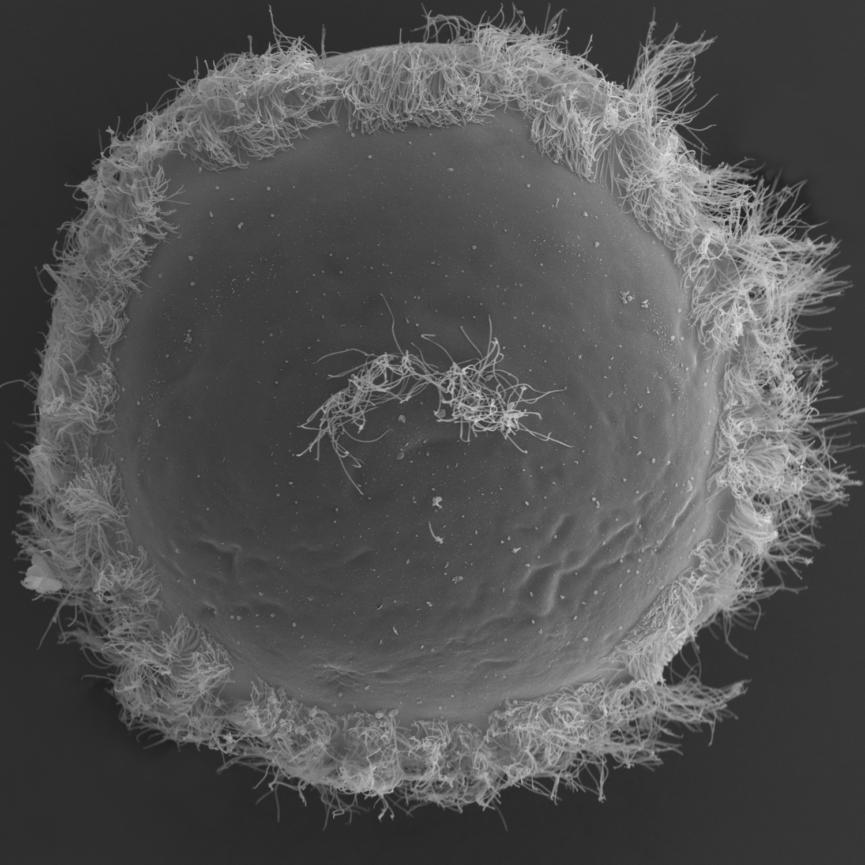
\includegraphics[width=.45\linewidth]{gfx/chapter1/platynereis_larva.jpg}} \quad
        \subfloat[Adult \platy{}. Image: Arendt group, EMBL]
        {\label{fig:platynereis_adult}%
         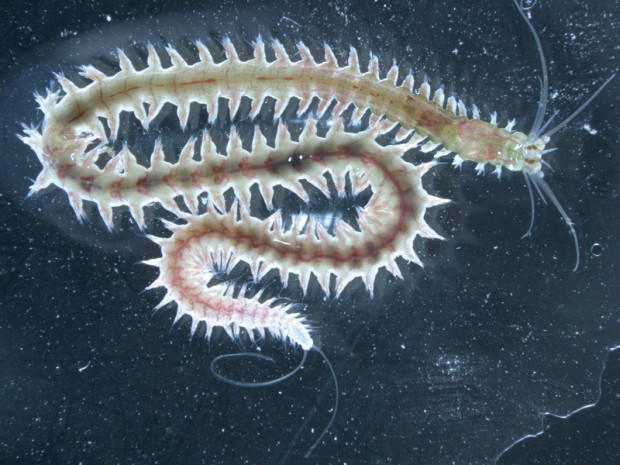
\includegraphics[width=.45\linewidth]{gfx/chapter1/platynereis_adult.jpg}}
        \caption{\platyfull{}'s larva and adult forms.}\label{fig:platynereis}
\end{figure}
     
     They are several reasons why \platy{} has been chosen as a model by numerous laboratories. In terms of evolution \platy{} shows several interesting characteristics. It belongs to the lophotrochozoan taxon of the bilaterian animals as opposed to most of the well established models animal which either belong to the ecdysozoans (\species{Caenorhabditis elegans}, \species{Drosophila melanogaster}) or the deuterostomes (mouse, human). Lophotrochozoans being extremely under represented, \platy{} as a model organism is essential to comparative approach on bilaterian biology.\\
     
     \platy{} also shows an exceptionally slow evolutionary lineage. It has even been described as a ``living fossil" for that reason \cite{Fischer10}. This means that the ancestral developmental characteristics of \platy{} are at an image of the common past of all bilaterians. To illustrate this fact an interesting example described in \cite{denes07,tessmar07} is the conserved molecular topography of the genes responsible for the development of the central nervous system between \platy{} and all vertebrates. This slow evolutionary rate confers \platy{} the advantage of being a link between fast evolving models like \species{drosophila} and vertebrates.\\
     
     In terms of practicality, \platy{} can easily be kept and bred in captivity producing offspring throughout the year \cite{fischer04}. The behavioural characteristics of \platy{} mating ritual have been well studied. The ``nuptial dance" happens on the water surface, male and female releasing the sperm and eggs synchronously, respectively. This activity is synchronized by pheromones released into the water \cite{zeeck98}. Over 2000 individuals can be produced within a single batch. Every new individual will undergo embryonic then larval development before reaching \platy{}'s adult form.\\

 
     \subsection{Larval development}
    Similarly to the other polychaetes, the larval development of \platy{} can be decomposed into three main anatomical stages: the trochophore, the metotrochophore and the nectochaete. The trochophore is spherical and moves via a equatorial belt of ciliated cells as well as an apical organ possessing a ciliary tuft \cite{rouse99,nielsen04} as seen on figure \ref{fig:platynereis_larvae} and schematically on figure \ref{fig:platynereis_larvae_scheme}. the metotrochophore stage is characterized by the development of a slightly elongated segmented trunk compared to that of the trochophore \cite{hacker98}. The next stage is the nectochaete larvae that resembles the adult (figure \ref{fig:platynereis_adult}) in most of the traits especially with parapodial appendages used for swimming and crawling \cite{hacker98}. This traditional subdivision has been applied to \platy{} \cite{hauenschild69}.\\
    
\begin{figure}[bth]
\begin{center}
  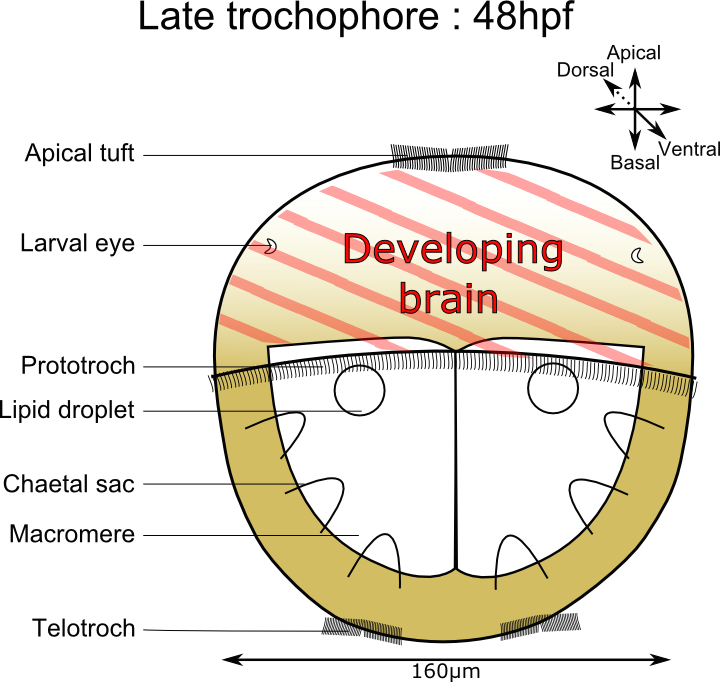
\includegraphics[width=0.6\linewidth]{gfx/chapter1/larvae48hpf.png}
\end{center}
  \caption{\platyfull{}'s larvea development at 48hpf or late trochophore. Striped in red is indicated the area which forms the developing brain of the larvae.}
  \label{fig:platynereis_larvae_scheme}
\end{figure}
    
    Aside from this purely anatomical subdivision, an additional staging systems exists and has become the norm for current studies. The development is measured in \textit{hours post fertilization} (hpf) at $18^{\circ}C$.
    
    A key factor making \platy{} such an interesting model to work with is the fact that after fertilization, the $\approx 2000$ larva will start developing at the exact same time, in a synchronous fashion. Furthermore, the larval development of \platy{} follows a very stereotypical pattern with very little variation from one individual to the other and even between batches provided the temperature is kept constant \cite{fischer04,dorresteijn90}. An example showing the similarity between individuals during development can be seen on figure \ref{fig:brain_comparison}. this is a very important feature as it allows biologists to repeat experiments on several individuals at a very close developmental stage even if they are from different batches.\\
    
\begin{figure}[bth]
  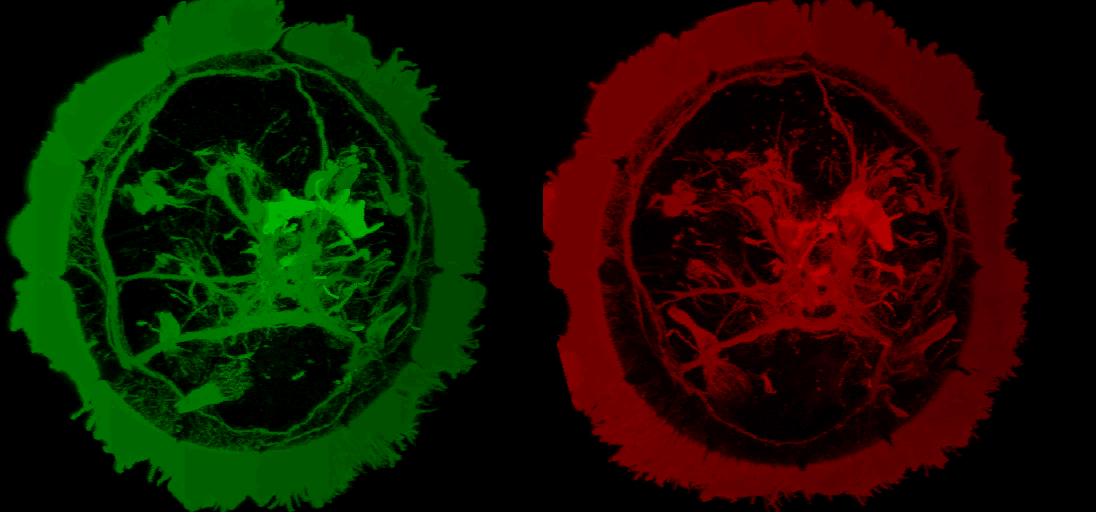
\includegraphics[width=\linewidth]{gfx/chapter1/brain_comparison.png}
  \caption{\platyfull{}'s stereotypical and synchronous development. In green and red are two different \platy{} individuals' with the same gene expression being highlighted. They show extremely similar patterns of development.}
  \label{fig:brain_comparison}
\end{figure}

	 Describing the entire development of \platy{} does not fall within the scope of this thesis. Indeed, we will only be interested in the brain of \platy{}'s larvae at 48hpf. Therefore, it is important to have an anatomical idea of what the brain looks like at this time in development and what inherent characteristics will be the most interesting to investigate.

\section{Gene expression in Platynereis' developing brain}\label{sec:gene_expression_background}
     \subsection{Platynereis' nervous development until 48hpf}
     The main purpose of this thesis is not to fully understand the patterns of development in \platy{}'s larval brain. Therefore we will only give a brief summary of what the main component of the brain are at 48hpf, the time point we will be interested in in the next chapters. \platy{}'s larval brain development is detailed in \cite{Fischer10}.\\
     From the early trochophore (24-26hpf) neural system development starts taking place. The apical ganglion forms at the apical tuft. It contains one sertonergic cell and a few neurons that link to the nerve of the ciliary band of the larva called the prototroch (see figure \ref{fig:platynereis_larvae_scheme} for better understanding). This allows the first movements of the larve thanks to the cialited cells of the prototroch.\\
     The mid-trochophore (26-40 hpf) sees the formation of the first cerebral commissure, it is a band of nerves interconnecting the ventral nerve cord and the brain. This trait is a typical feature of annelids brains. During this phase the apical ganglion becomes bigger with three more serotonergic cells.\\
     The late trochophore (40-48hpf)sees the formation of the second commissure in the ventral nerve cord. It is at the end of this stage that the brain starts to become more complexity with a notable increase in the number of neutrites.\\
     The data we will use in the rest of this thesis will not encapsulated the whole larvae, just the brain (see figure \ref{fig:platynereis_larvae_scheme}) thus excluding the ventral part of the nervous system. The best studied areas of the brain are the larval eyes, the developing adult eyes, the apical organ on the dorsal side. On the ventral side are located the mushroom bodies a pair of structures that are known to play a role in olfactory learning and memory in insects and annelids \cite{Tomer10}. A schematic representation of those areas is shown on figure \todo{FIGURE brain areas}.\\
     
     Even at a very early stage in a relatively simple organism, the brain quickly becomes a complex tissue. Cell types diverge and functional areas are formed. Before trying to understand more about \platy{}'s brain organization, it is interesting to ask the more general question about how complex tissues such as the brain are defined spatially.
     
          \subsection{Spatial organization of complex biological tissues like the brain}
     This section is not intended to demonstrate a specificity of the \platy{}'s brain, it is meant to ask some of the fundamental questions that intrinsically motivate the work presented in the rest of this thesis. Complex tissues, the obvious example of which is the brain, could be viewed as an interconnected mosaic of cells having different functions, working together to achieve the global function of the organ.\\
     
     If we look closely at this mosaic of cells, the spatial organisation of this mosaic is not random. Cells that serve the same function will often be close from each other, thus defining functional tissues. However, the spatial coherency of those tissues is not necessarily always the same. Some cell types could be formed of cells scattered inside another more spatially coherent tissue. To illustrate that fact, an interesting example is the difference between the spatial coherency of cells forming the neuronal tissue in the brain and cells forming a well defined region in the brain like the mushroom bodies. When asking the question, is it likely that this cell is fully surrounded by the same cell type, the extensions created by the axons of neurones will decrease this probability. Indeed, axons will grow through other types of tissues to reach their destination, making the overall spatial coherency of "neuronal" tissue smaller than very well spatially defined tissues.\\
     
     When trying to analyse the full structure of the brain with an automated method, keeping in mind that fact could prove important to improve the results. This fact and its consequences on the work presented in this method are further discussed in section \todo{cite section spatial clustering}.\\
     
     So far, we have only regarded organs and cell types as regarding their anatomical traits. But as mentioned in the introduction \ref{ch:introduction} the functional heterogeneity of complex tissues goes further that simple anatomical traits. We need to work on traits that fundamentally represent how cells are functioning.
     
     \subsection{Generalities about gene expression and development}  
     When speaking about developmental biology it it should be noted that the term ``cell" will be referring to eukaryotic cells and more specifically those of multicellular organisms. Every cell in a complex organism possesses the same genome, that is, the sum of all the genetic information contained in the cell (nucleus and other compartments). This fundamental homogeneity is in plain contradiction with the heterogeneity observed anatomically. If every cell has the exact same DNA, where does the great variability between cell types come from (what makes a neurone become a neurone and not a pancreatic cell). Answering this sort of questions defines the field of developmental biology.\\
     
     The short and rather complete answer to any developmental biology question actually is: same genome but different pattern of gene expression. As indeed gene expression is the central, most important, most studied cellular activity. Gene expression even is general common denominator of life as large parts of the mechanisms making up gene expression are actually shared by every living creature known to man.\\

     Of course to understand what gene expression is, we must first define what genes are. The precise definition of a gene is still controversial. The concept of a ``factor that conveys traits from parents to offspring" was laid by Gregor Mendel in 1866 \cite{mendel66} when the accepted theory at the time was based on blending inheritance where the traits of the parents appeared mixed in the offspring following a continuous gradient. The most recent published definition of a gene followed the publication of the ENCODE project \cite{feingold04}. It states that a gene is ``A gene is a union of genomic sequences encoding a coherent set of potentially overlapping functional products."\\

	Gene expression is the way cells express their genes. Expression of a gene is the process of transcribing the DNA of that particular gene. The product of gene expression is RNA molecules and there are several ways to look at gene expression. In a cell or tissue, at a given time point we can to choose to look whether a gene is expressed or not (binary expression) or how much a certain gene is expressed (quantitative expression).\\
	
	Most RNA molecules are translated into proteins that can have very different purposes some will directly serve in the cellular life as functional/structural agents (elements of the ATP synthase for example) others will have a regulatory effect on gene expression. In other terms the expression gene $a$, coding for protein $A$ might activate, accelerate, inactivate or decelerate expression of gene $b$ and potentially others. This outlines the complex interdependent regulatory system that is gene expression. For precise examples gene regulation see \cite{gossen92, shinozaki03,fuqua01,balmer02}.\\
	
	\todo{Add figure for gene expression Camille}
	
	During development mechanisms exist that allow gene expression to become differential as the divisions occur. This is how the asymmetrical axis (dorso-ventral, and basal-apical) of the body are defined. The main mechanism involves chemical gradients. The first of these gradient has to come from the original cell which musty contain some asymmetrically distributed chemical so that the first divisions lead to non identical cells. In the case of \platyfull{}, the body axis are defined  between 2hpf and 7hpf \cite{Fischer10}.\\
	
	As described, gene expression is the key factor during tissue development. The ability to study gene expression patterns has revolutionized the fields of developmental biology. Technological innovation has been the main driving factor of this revolution. In the next section we will present two methods to capture gene expression.


\section{Capturing gene expression in the laboratory}\label{sec:gene_expression_lab}
     \subsection{In-situ hybridization assays}
     In-situ hybridization (ISH) is an experimental technique where the practitioner is able to determine in which cells of the tissue under study a particular RNA is expressed. As opposed to Southern blotting, ISH assays not only allow to know whether a gene is expressed or not, but also where in the tissue it is expressed. First proposed in 1969 by Pardue \cite{pardue69} and John \cite{john69} independently, in-situ hybridization (ISH) used radioactive tritium labelled probes on a photographic emulsion to reveal on which chromosome particular genomic components were located. With the development of fluorescent labelling techniques \cite{landegent84,pinkel88} allowing for faster, more sensitive and of course safer hybridization assays \cite{swiger96} compared to radioactive probes, Fluorescent in-situ hybridization (FiSH) quickly became the standard technique to study gene expression in the spatial context of the biological tissue. Importantly, using multiple fluorescent probes of different colours allowed the simultaneous localization of several RNA fragments in the tissues \cite{nederlof89}.
     

     \subsection{Building a image library of gene expression for Platynereis}
     During his PhD, Raju Tomer and colleagues \todo{cite thesis} member of the Detlev Arendt lab in EMBL, used Fluorescent in-situ hybridization to create an image library of gene expression in the brain of \platy{}. He was able to record gene expression in the full brain at 48hpf for 169 genes. In practice each individual larvae was dissected to isolate the brain, which was then cut into thin slices and fixed. Each individual slice was then stained with two different fluorescent probes corresponding to two messenger RNAs (RNAm). One of the gene is considered a reference, as it is always hybridized in all the assays (the main reference gene used was Emx) along an other gene of interest, see figure \ref{fig:insitu}.\\
     
     As mentioned previously, the larval development of \platy{} is highly similar in every individual larvae. In the case of this study requiring a lot of different assays conducted each time a on different animal, the stereotypical development of \platy{} has proven essential. Indeed, having the same reference localized in all the assays has allowed Tomer to align all the other gene expression patterns onto this scaffold.\\
     
     The result is an image library of 169 gene expression pattern in the full brain of \platy{} with a exploitable spatial reference that allows for a very precise mapping.
    
    \begin{figure}[bth]
\centerline{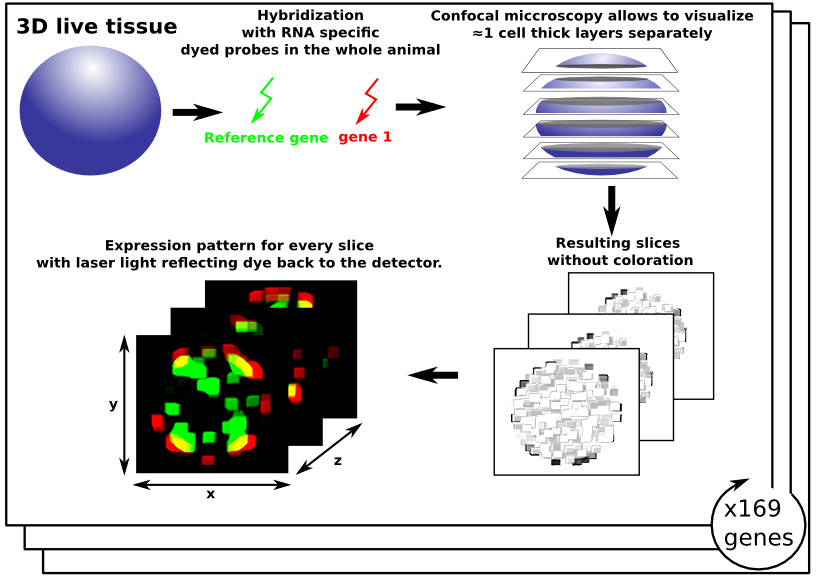
\includegraphics[width=0.9\linewidth]{gfx/chapter1/insitu.png}}
\caption{Fluorescent in-situ hybridization assays to create a 169 genes catalogue of gene expression in the brain of \platy{}. From the live tissue cut into thin fixed layers, every slice is stained with a reference gene and a gene of interest that will reveal the areas of expression under fluorescent microscopy. The process repeated 169 times for key genes in \platy{} development has been generated by \cite{Tomer10}}\label{fig:insitu}
	\end{figure}
	
	However useful and practical fluorescent in-situ hybridization may be, such assays are limited in terms the quantity of gene one is able to study. Indeed, each individual larvae only provides the expression of two genes, one being the reference. Crucial developments in sequencing technologies have brought a way to study the expression of the whole transciptome landscape in a single assay, RNA sequencing.

     \subsection{RNA sequencing}
     Whole Transcriptome Shotgun Sequencing (WTSS) also called RNA sequencing (RNA-seq) \cite{morin08,wang09} has developed alongside Next Generation Sequencing (NGS) technique used to retrieve the genome (DNA). Instead, when preparing the starting material, only the RNAs are extracted. If interested in protein coding messenger RNA, they are separated from the rest by targeting the polyadenylated 3' tail, specific to protein coding transcripts. Most current technique use magnetic beads to achieve this separation \cite{mortazavi08,morin08}.\\
     
    Once isolated from a population of cells, transcripts undergo fragmentation to obtain an average length of 200-300. The next step is then reverse transcription, which will create a complementary DNA (cDNA) library using a viral reverse transcriptase enzymes. After amplification using quantitative Polymerase Chain Reaction (qPCR), the cDNA library is ready to be sequenced by NGS technology.\\
    
    This will generate a large dataset of small reads, that need to be mapped back onto the reference genome of the considered species, providing this genome is available. In that case the resulting dataset will reflect a snapshot of the whole transciptome in the studied cell population. However, in the case of \platy{}, this reference genome is not fully available yet, an alternative option being to map the reads back to a list of known gene sequences, for instance the 169 genes studied by \cite{Tomer10} (PrimR genes). The obtain dataset will represent a quantitative image of the considered genes in the cell population at one point in time.\\
    
    Because of technical limitations in this sequencing protocol, until very recently the starting quantity of RNA had to be relatively important. This is why most of the published RNA sequencing studies use a population of cell as a starting point. This however, means that the gene expression landscape obtained as an output will represent an averaged expression over all the cells used as an input.\\
    
    Importantly, when comparing RNA-seq the the previously described in-situ hybridization technique, if the methodological burden to analyse the expression of a lot of genes at the same time is greatly reduced, the spatial localisation of the cells is lost during the protocol.\\
    
\section{Conclusions}
     
     In this chapter we have presented \platyfull{} and the advantageous traits it exhibits for developmental biologists especially in the field of neural development. We have discussed the fact that anatomical traits are not sufficient to fully comprehend the deep heterogeneous patterns of functionality inside a complex organ such as the brain. In order go push this understanding further we need to take an interest in what defines the life of tissues and sub-tissues, gene expression. We have also described two methods that allow practitioners to capture gene expression from a biological tissue, and how an image library  of gene expression for 169 gene was generated by \cite{Tomer10} in the full brain of \platy{}.\\
     
	So far, our scale of study has been the tissue, or the sub-tissue. However, as mentioned in the introduction \ref{ch:introduction}, the heterogeneity of complex biological tissues does not stop at this scale of study. In fact, with a top-down approach looking at big tissue and then separating them in smaller sub-tissues until ``true" functional tissues are defined is an extremely complicated approach. A solution to this problem would be to actually reverse the approach from a top-down to a bottom-up mindset. This mean reducing the scale of study to the smallest biological unit we can work with, the single cell, define the heterogeneity of gene expression at the single cell level and work our way up to the functional tissue level. Instead of a fragmentation problem, we would have a clustering problem, attaching single cells to a certain number of categories. In order to implement such an approach, what we need is single cell gene expression data.

%
%
%
%
%





%*****************************************
\chapter{From tissue to single cell transcriptomics, a paradigm shift}\label{ch:singlecell}
%*****************************************
\section{Spatially referenced single cell-like in-situ hybridization data}\label{sec:single_cell_insitu}
  \subsection{Dividing images into ''cells''}
  Because in-situ hybridization preserves spatial information in the tissue under study, measuring gene expression at single cell resolution from an image obtained through confocal microscopy is a matter of microscope performance and cell size. For big enough cells, single cell resolution has been documented as far back as 1989 \cite{tautz89,poulsen93}.\\
  
  When considering the \platy{} brain dataset, with current microscope technology, achieving single cell level resolution on one particular image is feasible. However, the main limitation is analysing the quantity of data involved; indeed, each brain is separated into 20 slices, for 169 genes this yields 3380 images that require inspection. This technical bottleneck can be overcome with an automated way of analysing the fluorescence images. However this is not an easy task, as the computer program required needs to be able to \emph{see} and divide the global picture into cells. Considering that all cells do not exhibit the same shape and size, constructing this \emph{cell model} is a very complicated task.\\
  
  It is for instance possible to highlight the limits of the cells and to automatically acquire those boundaries through computer vision methods. This process relies on targeting proteins in the membrane or in the extracellular matrix of the cells with specific fluorescent probes. Once the boundaries are acquired, defining every cell is a matter of finding enclosed spaces. To that end, numerous contour detection algorithms exist \cite{li95,fan01,arbelaez11}.\\
  
  Unfortunately, a dataset with the cell limits highlighted does not yet exist for \platy{}'s brain, making a precise division of the images into cells very difficult. Instead, Tomer used a simple approach that divides the images into ``cubes'' \cite{Tomer10}.


  \subsection{A simple cell model, the ''cube'' data}
  
  Every slice of \platy{}'s brain being aligned onto the reference gene scaffold (see section \ref{sec:gene_expression_lab}) for all 169 genes, the ``cube'' model simply consists of dividing each image into squares approximately the size of an average cell. In the \platy{} dataset, the size chosen was 3 \microm{2} \cite{Fischer10}. Importantly, this is actually smaller than the average cell size in \platy{}'s brain. Each slice of the brain being approximately 3 \microm{} thick, the resulting dataset, spatially referenced in 3D, will contain 3 \microm{3} cubes, each of which is associated with the luminescence data for each of the 169 genes.\\
  
  Of course this cell model is far from perfect: it assumes that every cell in the brain is roughly the same size and cubical, which is clearly not the case. Consequently, the ``cube'' model will introduce errors in the dataset. The first type of error occurs within areas where the genes under study are highly expressed. In that case, the light emission might contaminate the surrounding cubes that do not necessarily express the same gene (see Figure \ref{fig:cubeserrors}A). The second type of error is introduced by the choice of 3 \microm{3} cubes. As they are smaller than the average cell, some cubes will fall on areas that may be artificially empty. Indeed, transcription in the cells mainly happens in the nucleus. mRNA molecules then travel to the cytoplasm to be translated but they are not evenly distributed across the cell; in particular for some large cells, parts of the cytoplasm may record no expression in a cell that actually contains a lot of transcripts (see Figure \ref{fig:cubeserrors}B).\\
  
  Hence, the data will tend to exhibit spatial discontinuity and inconsistency. With this fact in mind, any automated way of interpreting this data (in the case of this thesis: clustering ``cubes'' into cell types) will have to take into account this spatial discontinuity and try as much as possible to smooth over those potential expression gaps.\\
  
    \begin{figure}[h]
\centerline{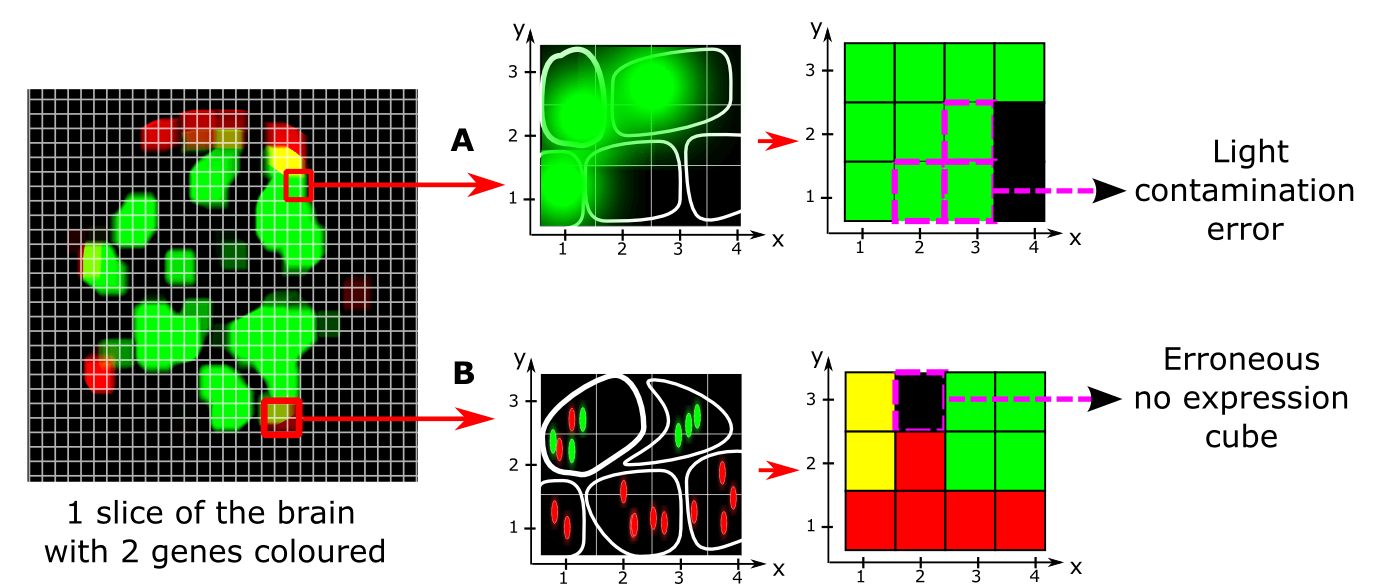
\includegraphics[width=1.3\linewidth]{gfx/chapter2/cubeserrors.png}}
\caption{Errors introduced by the ``cube'' cell model. Path A shows how regions with highly expressed genes can introduce errors through light contamination. Path B shows how some cubes may appear artificially void of expression because of the uneven distribution of transcripts inside the cytoplasm especially for large cells.}\label{fig:cubeserrors}
	\end{figure}
	
	However, even with this simple cell model, the data generated by \cite{Tomer10} is highly valuable. Indeed, not only does this dataset give a snapshot of gene expression for 169 genes in the full brain of \platy{}, it also attaches spatial information to each data point.\\

\section{Single cell RNA sequencing, building a map of the full transcriptome}\label{sec:single_cell_rnaseq}
  \subsection{Single cell RNA sequencing}
	The scale shift from tissue to single cell is harder to achieve in the case of RNA-seq. As described in the Introduction \ref{sec:gene_expression_lab}, an important factor for the success of RNA-seq assays is the input quantity of RNA to be sequenced. Taking mammalian cells as a reference, the quantity of RNA depends a lot on the cell type considered and can vary between 10 and 50 pg per cell, only 2\% of which is mRNA \cite{iscove02,islam11}. With such a small input quantity, distinguishing biological variation between different cells from the technical variation linked to mRNA capture rates and to cDNA amplification protocols is extremely challenging.\\

	However, with the creation of new protocols \cite{ramskold12,tang09}, and the rise of microfluidics approaches that faciliate the extraction and sequencing of single cells \cite{ozsolak10}, the last couple of years have seen a dramatic increase in the number of single cell RNA-seq based studies \cite{islam13,marinov13,yan13,staahlberg13,deng14}. However, challenges still need to be overcome in order to analyse further complex tissues using such approaches.

  \subsection{Mapping back gene expression to a spatial reference}

	Single cell RNA-seq captures a snapshot of the entire transcriptome of a given cell at a given point in time. However, to analyse cells from a complex tissue, current protocols require that the tissue be reduced to a suspension of single independent cells. This prevents the user from keeping track of any spatial information about the cells. Hence, when analysing single cell RNA-seq data from a complex tissue, back-mapping every cell to its original location becomes a crucial problem.\\ 
	
	A recent paper published in Cell \cite{durruthy14} describes a purely mathematical way to approximate the spatial organisation of sequenced single cells using a series of statistical methods to segregate and map single cells RNA-seq data obtained from mice otocysts onto a reference sphere. The method mainly based on Principal Components Analysis, allows them to reconstruct a ``image'' of the otocyst.\\
	
	To push the method presented in \cite{durruthy14} further, we could achieve back-mapping of the single cells to a different dataset with a spatial reference. This reference should consist of an independent assay where gene expression in the considered tissue is defined for enough genes at a spatially small enough resolution to find for each sequenced cell, if not its exact original location, at least a restricted region of the tissue from which the sequenced cell originated with a high probability.\\
	
	Fortunately, in-situ hybridization assays provide exactly this type of data and I will present in the last section of this Chapter (\ref{sec:back_mapping_platy}) a methodological proof-of-concept of this back-mapping in the brain of \platy{} with 72 sequenced single cells. However, before that, I will discuss the impact of the noise level in both in-situ hybridization and single cell RNA-seq assays on the quantitative nature of the resulting datasets.

\section{About the quantitative trait of single cell expression data}\label{sec:quantitative_single_cell}
  \subsection{Light contamination in in-situ hybridization data}
  The light intensity value obtained from in-situ hybridization assays can be considered as a quantitative measure of gene expression \cite{dorresteijn90}. Indeed, the light emitted by every cell in the considered tissue is correlated with the number of RNA fragments of the gene of interest present in the cell as each fragment bound to a probe is an independent source of emission and the probes are hybridized in the cells in large excess. This means that if the targeted gene is highly expressed in a cell, there will be more sources of emission, thus making the overall light intensity captured on this area higher than in a cell expressing the gene at a low level. \\
  
  As mentioned in Section \ref{sec:single_cell_insitu}, in-situ hybridization assays at the single cell level are prone to localized errors due to the cell model. One explanation for those errors, as shown in Figure \ref{fig:cubeserrors}B is the phenomenon of light contamination. When a large group of neighbouring cells express the same gene, the additivity of light intensity mentioned above means that even though the cells express the gene at the same rate, cells surrounded by a lot of other cells expressing the same gene will have abnormally high light intensity readings due to light contamination from the adjacent areas. As a result, when considering a hypothetical circular portion of tissue where a gene is monotonously expressed, the recorded light intensity will show a gradient with the maximum localized on the circle's centre.\\
  
   \begin{figure}[H]
\centerline{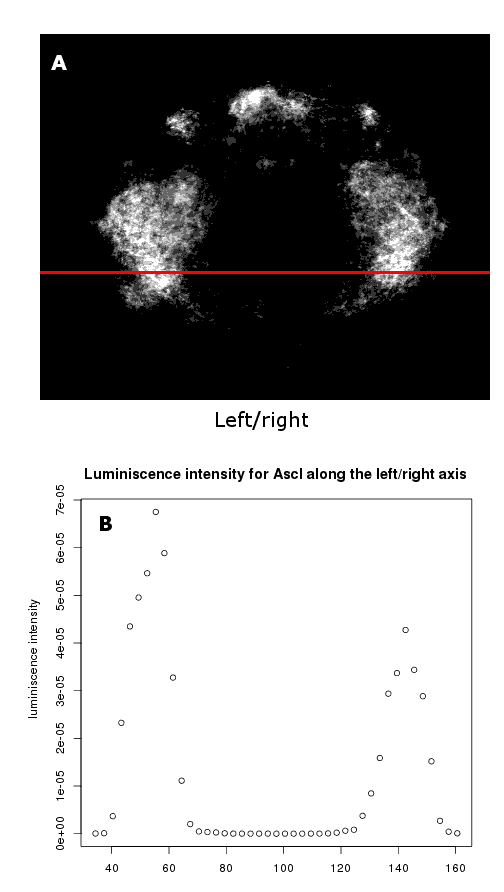
\includegraphics[width=0.8\linewidth]{gfx/chapter2/whybina.png}}
\caption{{\bf Light contamination in in-situ hybridization luminescence data seen with the example of the gene Ascl.} Panel A shows the raw fluorescent microscopy capture of the gene's expression for one layer in the brain of Platynereis. Panel B shows the light intensity measured along the red line in panel A. Because of the small scale of study, cells surrounded by other cells expressing a particular gene will have higher intensity values because of nearby light contamination.}\label{fig:why_binarize}
	\end{figure}
  
  As shown in Figure \ref{fig:why_binarize}, the issue of light contamination seems to occur when using the 3 \microm{3} ``cube'' model. In this context, and because of the single cell scale of this study, considering the in-situ hybridization data as quantitative may introduce significant errors. In order to avoid this light contamination bias a solution is to transform the quantitative data into binary data where, for a given ``cube'', genes are simply expressed or not.
  


  \subsection{Technical noise in single cell RNA-seq data}
  Single cell RNA-seq is also prone to high levels of noise. This technical noise is caused by the minute amounts of starting RNA material. A study led by Philip Brennecke, Simon Anders and Jong Kyoung Kim \cite{brennecke13}, proposes a statistical method to overcome this high noise level and distinguish between biological variation and technical variation in the gene expression levels.\\
  
  To illustrate the dramatic increase in noise level, they used a series of dilution assays, reducing step by step (5000 pg, 500 pg, 50 pg, 10 pg) the input quantity of RNA fragments extracted from total \species{Arabidobsis thaliana} RNA with two technical replicates each time using the single cell RNA-seq Tang protocol \cite{tang09}. The authors of the study let me analyse this data, and after normalizing by the size factor using the Bioconductor package DESeq \cite{anders10} the scatter plots shown in Figure \ref{fig:dilutions} were generated. \\
  
  It is clear from these dilution assays that the noise level is correlated with the input quantity. Even though highly expressed genes are consistently well quantified even with 10 pg input material, for most of the genes, with less than 50 pg input RNA it seems dangerous to assume the results of single cell RNA-seq as quantitative with the current technological capabilities.
  
\begin{figure}[h]
        \myfloatalign
        \subfloat[500 pg input RNA.]
        {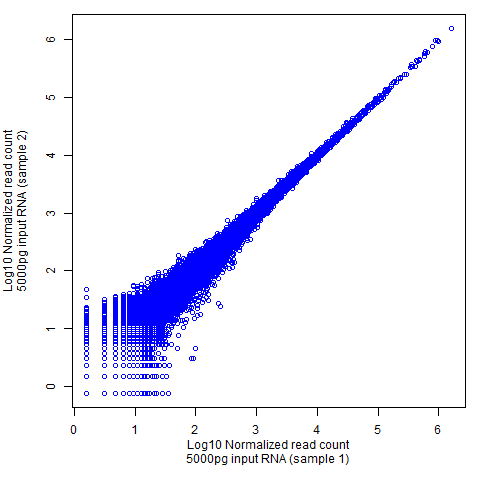
\includegraphics[width=.45\linewidth]{gfx/chapter2/5000pg.png}} \quad
        \subfloat[500 pg input RNA.]
        {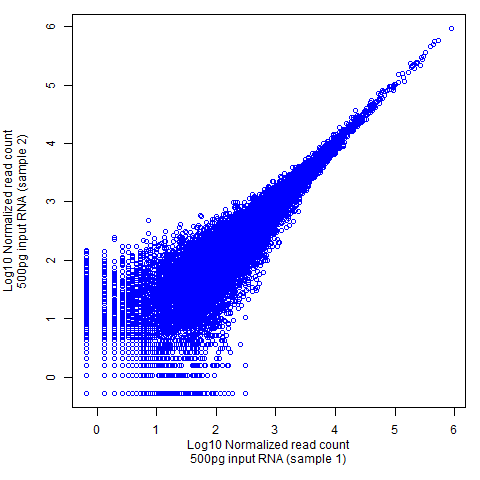
\includegraphics[width=.45\linewidth]{gfx/chapter2/500pg.png}} \\
        \subfloat[50 pg input RNA.]
        {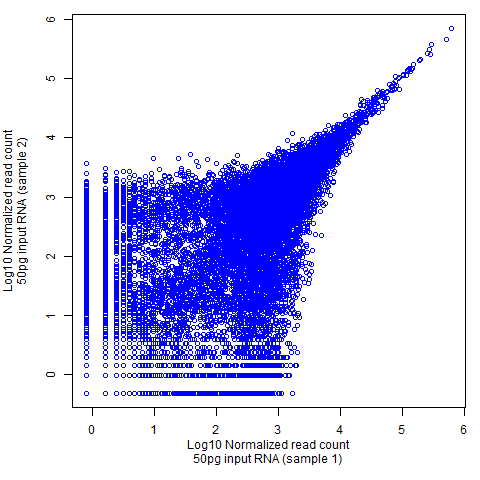
\includegraphics[width=.45\linewidth]{gfx/chapter2/50pg.png}} \quad
        \subfloat[10 pg input RNA.]
        {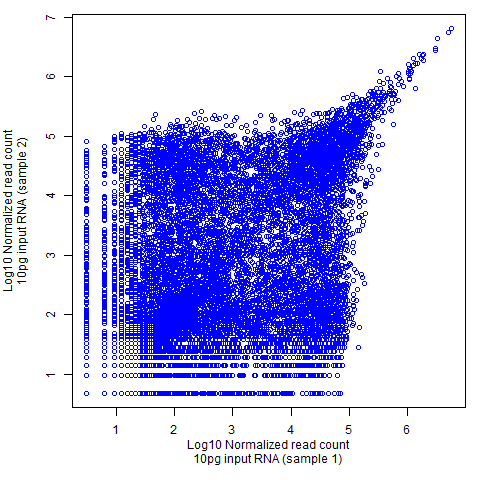
\includegraphics[width=.45\linewidth]{gfx/chapter2/10pg.png}}
        \caption{Dilution series of total A. thaliana RNA}\label{fig:dilutions}
\end{figure}


	The paragraphs above have shown that neither in-situ hybridization nor RNA-seq data are fully quantitative when the scale is lowered to the single cell level. To avoid problems linked to the noise level in the rest of this study, a solution was to binarize single cell datasets. However, binarization is not a trivial problem as discussed in the following section.
	
	
  \subsection{Binarizing in-situ hybridization datasets}
	As shown in Figure \ref{fig:why_binarize} and discussed in the previous section \ref{sec:quantitative_single_cell}, the various problems linked to light contamination can be avoided by transforming the ``quantitative'' fluorescence information into binary data. In other words, if $S$ is the set of all ``cubes'' in the brain, $M$ the set of all the considered genes and $y_{i,m}$ the value retrieved from the in-situ hybridization data for ``cube'' $i \in S$ and gene $m \in M$, then  $y_{i,m} = 1$ if gene $m$ is expressed at site $i$, $y_{i,m} = 0$ otherwise. The binarization process itself is not trivial. Indeed, defining the light intensity threshold above which a gene is considered expressed is a complicated problem, especially for noisy data.\\

	Looking at the density of intensities across all the ``cubes'' for each gene yielded two very different scenarios: some densities were separated into two clear peaks, making the threshold easy to find while others exhibited a single peak making it hard to choose a clear cut value as shown in Figure \ref{fig:densities_bina}. After trying different thresholding methods based on those densities, I found, in collaboration with Kaia Achim and Maria Tosches from the Arendt group in EMBL Heidelberg that none of them resulted in binary expression that was satisfying for many genes when compared with a manual inspection of the in-situ hybridization raw images. Considering that this binarized dataset will be the cornerstone of the work presented in this thesis, it was very important to achieve a high confidence thresholding. Given the small number of genes studied (169), and the collaboration with a team of biologists working specifically on \platyfull{}'s brain, a manual thresholding approach was developed. Indeed, by going through the 169 genes one by one, it was possible to adjust the thresholds manually until the resulting binarized expression pattern corresponded perfectly to 1) the fluorescent stack images from in-situ hybridization data; 2) the biologically known expression patterns in the brain of \platy{} expected by the biologists.\\
	
	\begin{figure}[H]
\centerline{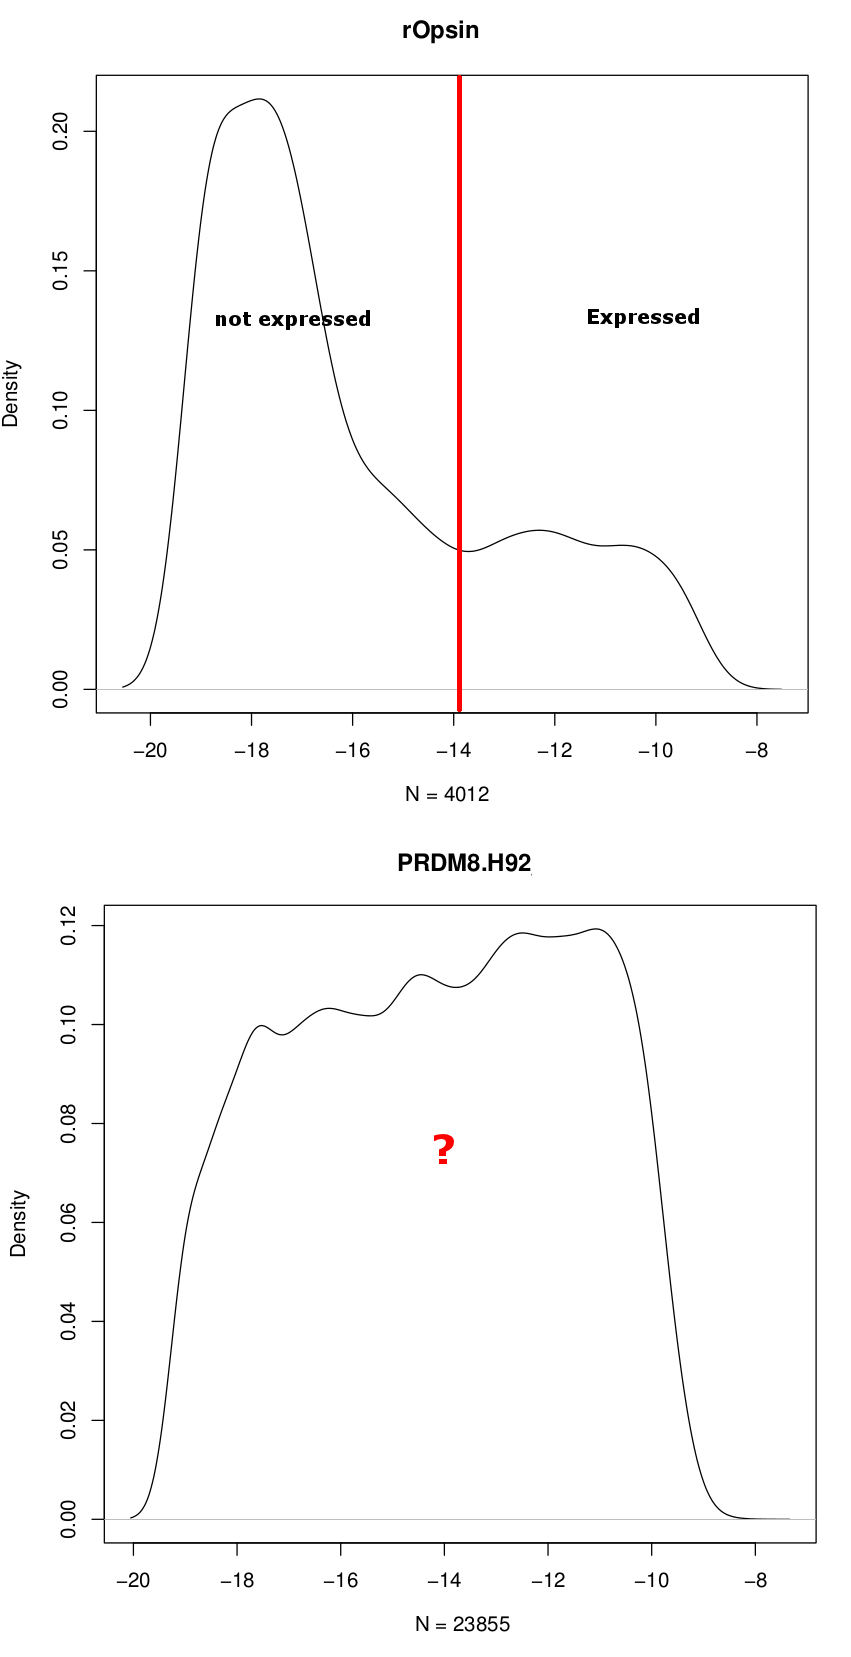
\includegraphics[width=0.8\linewidth]{gfx/chapter2/densities_bina.png}}
\caption{{\bf Densities of log luminescence values for two genes (rOpsin, PRDM8) over the $32,302$ cells.} For {\it{rOpsin}}, the density exhibits two clear peaks making the choice of a binarizing threshold easy. By contrast, for {\it{PRDM8}} there is no such clear threshold, making an automated binarization method hard to implement.}\label{fig:densities_bina}
	\end{figure}
	
	This method resulted in a high confidence binarized dataset for $86$ genes. Several reasons explain why $83$ genes out of the starting $169$ were removed from the dataset. For some of the genes no good threshold could be found, this was due to high noise level in the in-situ hybridization images. Other images suffered from experimental errors that yielded blurred and unexploitable expression patterns. Finally some images were polluted by a well known experimental artefact linked to confocal microscopy imaging as shown in Figure \ref{fig:artefact}.\\
	
\begin{figure}[h]
        \myfloatalign
        \subfloat[Z-stack of gene Smad23 showing an experimental artefact (round very bright spot in the middle).]
        {\label{fig:hist_rna}
        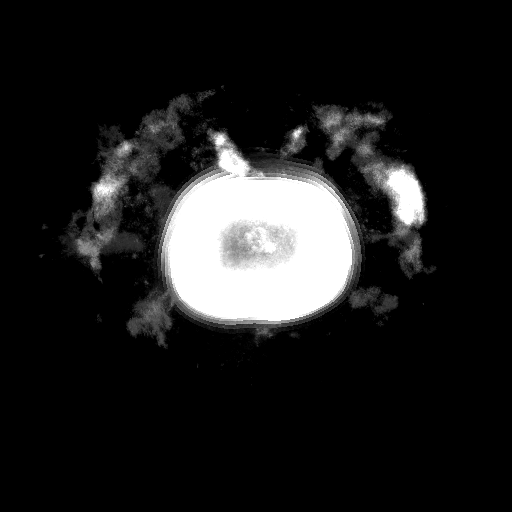
\includegraphics[width=.45\linewidth]{gfx/chapter2/smad23.png}} \quad
        \subfloat[Z-stack of gene Syt showing an experimental artefact (round very bright spot in the middle).]
        {\label{fig:density_rna}%
         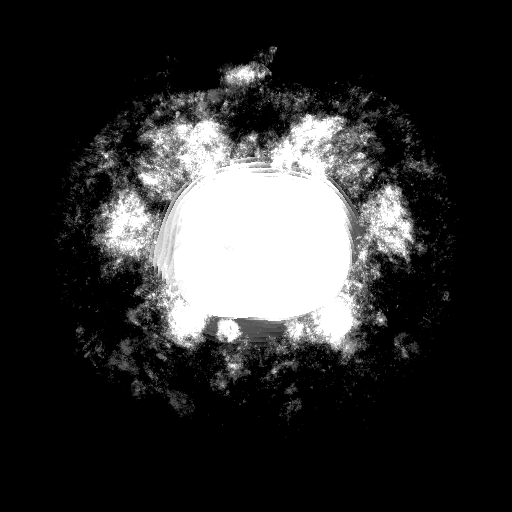
\includegraphics[width=.45\linewidth]{gfx/chapter2/syt.png}}
        \caption{Confocal microscopy experimental artefact for 2 genes of the original $169$ studied genes.}\label{fig:artefact}
\end{figure}
	
	Although the aforementioned method resulted in a high quality binary dataset, it has been possible only because the number of genes considered was small. This will not be the case when dealing with RNA-seq data.
	
\section{Preliminary results on single cell RNA-seq in \platy{}'s brain}\label{sec:back_mapping_platy}
  \subsection{Single cell RNA-seq in Platynereis' brain}
  
    	A collaborations with Kaia Achim in the Arendt lab in EMBL provided us with a unique RNA-seq dataset of 72 single cells from \platy{}'s 48hpf developing brain. 
    	
	Experimentally, the work consisted in setting up \platy{} batches, picking up 50-100 individuals at 48hpf. These were washed in Ca-Mg free sea water and incubated in a mixture of pronase which breaks extracellular matrix and thioglycolate (helps to break the chorion). After this treatment, the trunks and epispheres (brains) were separated. 40-60 epispheres were then picked out, transferred to Phosphate buffered saline (PBS) and then incubated for 1 minute in PBS containing collagenase to break more extracellular matrix. After two PBS washes, the cells were dissociated by pipetting up and down then washed again in 1 ml of PBS and concentrated by centrifuging (1 min, 1000 rpm). Cells were re-suspended in 20 microliters of PBS, of which 5 microliters could be loaded on the capture chip.\\

	Fluidigm's C1 Single-Cell Auto Prep System instrument with the Fluidigm Single-Cell Auto Prep IFC chip optimized for 10-17 micron cells were used as shown in Figure \ref{fig:singlecell_chip}. The reverse transcription was performed using Clontech SMARTer Ultra Low Input RNA Kit and for on-chip PCR the Clontech ADVANTAGE-2 PCR kit. Sequencing libraries were prepared using Nextera DNA Sample Preparation kit from Illumina.\\
	
\begin{figure}[h]
        \myfloatalign
        \subfloat[Fluidigm C1 chip with 96 wells. Image taken from Fluidigm website]
        {\label{fig:c1}
        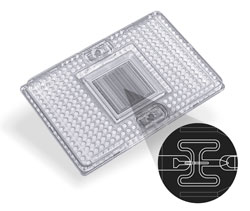
\includegraphics[width=.45\linewidth]{gfx/chapter2/c1.jpg}} \quad
        \subfloat[One cell from \platy{}'s brain captured in the chip (circled in red). Image generated by Kaia Achim]
        {\label{fig:chip}%
         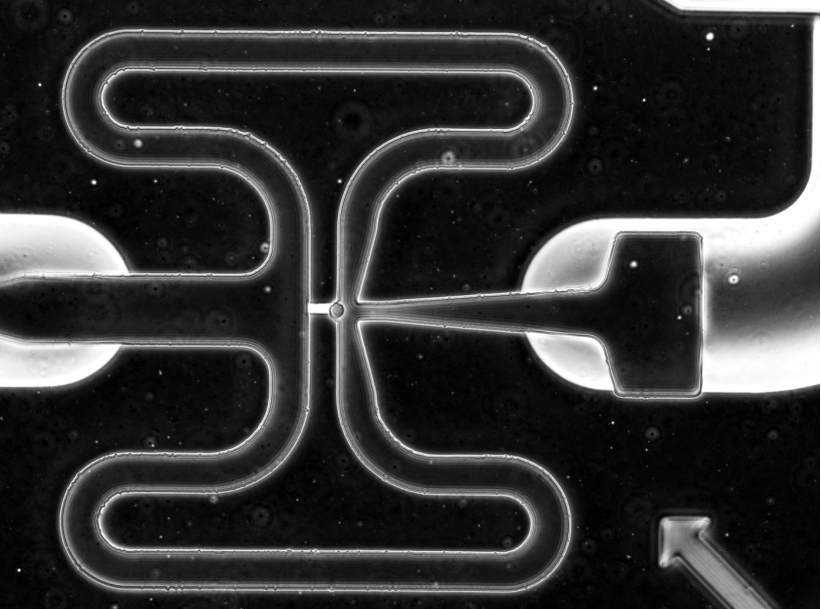
\includegraphics[width=.45\linewidth]{gfx/chapter2/chip.png}}
        \caption{Microfluidics single cell sequencing with C1 chips.}\label{fig:singlecell_chip}
\end{figure}
	

	With two chips and a capture rate of 65\%, 72 libraries were sequenced including 11 cells from first chip. From the second chip 35 live single cells, 17 dead single cells, 3 wells containing 2 cells, one with 4 cells, and 3 unsure ones resulting in 72 raw reads files as shown in Table \ref{tab:rna_seq_res}.\\	
	
\begin{table}
    \myfloatalign
  \begin{tabularx}{\textwidth}{X|c} \toprule
    Chips used & 2 \\
    Capture rate  & 65\%\\
    Libraries sequenced & 72 \\
	Live single cells & 38 \\
	Dead single cells & 15 \\
	Debris + live single cell & 4 \\
	Multiple cells & 6 \\
	Debris/unsure & 9\\
  \end{tabularx}
  \caption{Results over two C1 chips. The experiments were conducted by Kaia Achim.}\label{tab:rna_seq_res}
\end{table}
  	
	Of course those results do not include the spatial localization of the cells as the protocol requires the separation of the coherent tissue into a cell suspension. As a crucial point in any dowstream analysis, being able to map back the single cells to their original location in the brain is required. To that end, I took advantage of the spatially localized in-situ hybridization described in the previous section.\\


  \subsection{Mapping RNA-seq data back to PrimR in-situ hybridization assays}
  	Firstly, Bowtie \cite{langmead12} was used to map the RNA-seq raw reads to a reference containing the sequences of the 86 reference genes composing the in-situ hybridization data. The resulting dataset comprises the number of reads mapped back to each of the 86 genes in the 72 cells sequenced (Figure \ref{fig:backmap}).\\
  	
  	 In order to map back to the in-situ hybridization data, the chosen approach consisted of extracting the genes that were the most specifically expressed for each sequenced cell, before comparing this specific fingerprint to the in-situ 3D data in order to isolate the regions of the brain where those specific genes are co-expressed.\\
  	
	\begin{figure}[h]
\centerline{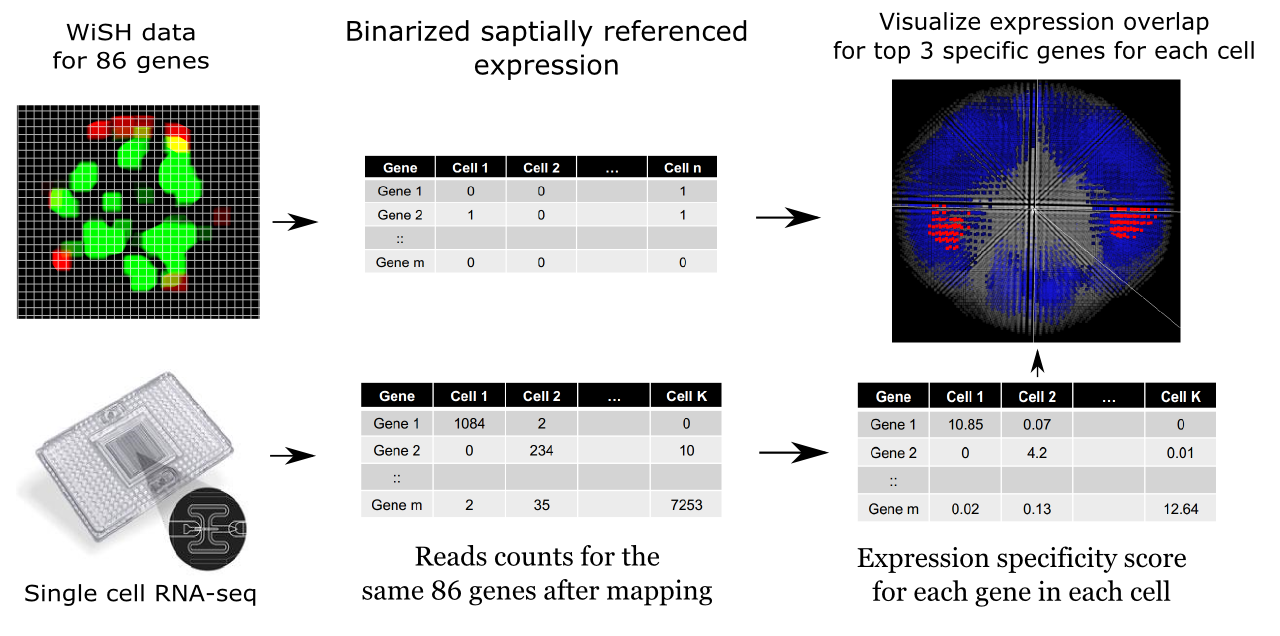
\includegraphics[width=1.5\linewidth]{gfx/chapter2/backmap.png}}
\caption{{\bf Spatial back mapping of single cell RNA-seq.} The binarized in-situ hybridization data provides the spatial reference onto which the single cell results will be mapped. All the single cells sequenced are put together and a expression specificity score for each gene and each cell is computed. Tha mapping is realized using the top 3 or 4 most specific genes for each cell.}\label{fig:backmap}
	\end{figure}
	
	Given the set of 86 considered genes $M$, and the set of 72 cells $C$, with the read count matrix $D$ of size $M\times C$, the expression specificity ratio $r_{m,c}$ can computed for each cell and each gene as :
\begin{eqnarray*}
	r_{m,c} &= \frac{D_{m,c}}{\frac{1}{\left\|C\right\|}\sum_{a \in C}D_{m,a}}
\end{eqnarray*}
where $\left\|C\right\| = 72 $ is the number of cells considered. Subsequently, for each cell, the genes with the highest specificity scores can be determined. On the one hand, this method has the inconvenience of using the average expression level across all considered cells to compute the ratio $r$. This means that the ability to precisely infer the original location of each cell, in other words, the mapping quality will depend on the overall sequencing quality. Furthermore, this method's performance relies on the assumption that the data are in fact a collection of cells from different cell types. However, given the experimental protocol described above, this seems to be an acceptable hypothesis. On the other hand, this mapping method has the advantage of not being sensible to technical noise in the RNA-seq protocol, providing the technical noise between cells remains at a constant level. This justifies the use of read counts in a quantitative way and not as binarized dataset.\\

	The goals of this study were to validate the protocol used in order to obtain single cell RNA-seq results in \platy{}'s brain and to establish a methodological proof-of-concept on spatially mapping RNA-seq results onto in-situ hybridization data. I will present here a few examples of sequenced cells, their most specifically expressed genes and their resulting potential original location in the brain as well as the probable cell type they belong to.\\
	
	In Table \ref{tab:rna_seq_representative_genes} are shown the most specific genes for four of the sequenced cells. For each cell, this list of genes can be used to visualize the areas within the brain where they are co-expressed according to the in-situ hybridization data. A snapshot of this visualization is shown on Figure \ref{fig:cell_localization}. In every case, simply looking at the three most representative genes seems to allow a clear localization of the sequenced cells. Of course this mapping is not at the single cell level, but having an idea of the tissue every cell originated from is already a nice proof-of-concept.\\
	
	From the most specific genes to each cell and their potential localization, it is possible to hypothesize, using previous biological studies, the cell type of each sequenced cell. As shown in Table \ref{tab:rna_seq_representative_genes}, for cell ``X2C911L'' the most specifically expressed gene ``Emx'' has been used as a reference gene to localize the mushroom bodies, a hypothesis which is compatible with the co-expression of ``CALM.R29'' and ``Dach'' \cite{Tomer10}. Cell ``X2C521L'' expresses Wnt8 very specifically, a gene shown to be linked to lateral brain development. Cell ``X2C61L'' can be easily classified as a developing neuron. Indeed both VACht (Vesicular acetylcholine transporter) and ChaT (Choline acetyltransferase) are genes coding for enzymes interacting with the neurotransmitter acetylcholine. Finally cell ``X2C241S'' displays the specific expression of the gene ``Mitf'', one of \platy{} most studied gene and expressed solely in the developing adult eyes \cite{kozmik08,guy08}.
	
\begin{table}
    \myfloatalign
  \begin{tabularx}{\textwidth}{X|X|X|X} \toprule
    \tableheadline{X2C911L} & \tableheadline{X2C521L} & \tableheadline{X2C61L} & \tableheadline{X2C241S} \\ \midrule
    Emx & Wnt8 &  VAChT & Mitf\\
    CALM.R29 & HEN1-Y61 & ChaT & Otx\\
	Dach & Gsx & LYamide & Tolloid-Y68\\
    
\midrule
	Mushroom body & Developing lateral brain & Differentiated neural tissue & Adult eye\\
    \bottomrule
  \end{tabularx}
  \caption{Top 3 most specific genes for 4 sequenced cells and the potential tissue they belong to. The resulting localization of those four cells infered from the in-situ hybridization data are shown in Figure \ref{fig:cell_localization}.}\label{tab:rna_seq_representative_genes}
\end{table}

\begin{figure}[H]
        \myfloatalign
        \subfloat[X2C911L: Emx, CALM.R29, Dach]
        {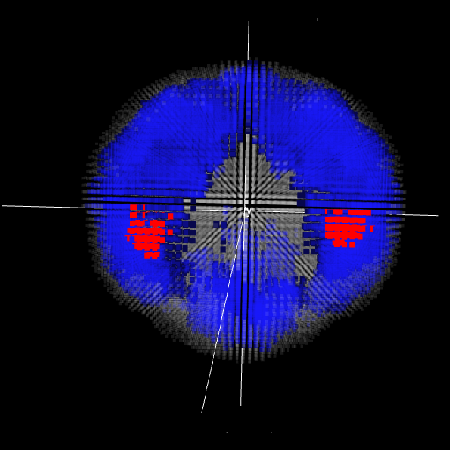
\includegraphics[width=.45\linewidth]{gfx/chapter2/cell1.png}} \quad
        \subfloat[X2C521L: Wnt8, HEN1-Y61, Gsx]
        {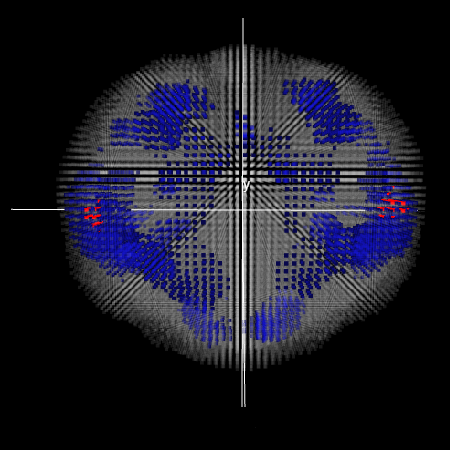
\includegraphics[width=.45\linewidth]{gfx/chapter2/cell2.png}} \\
        \subfloat[X2C61L: VAChT, ChaT, LYamide]
        {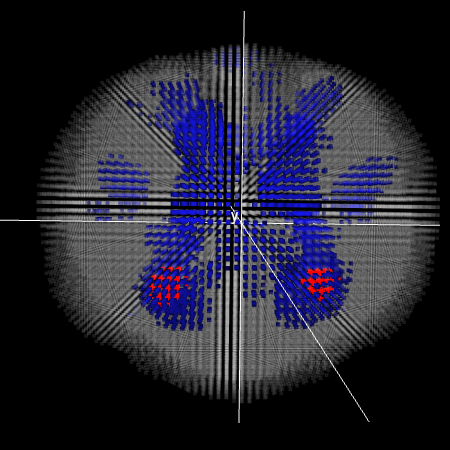
\includegraphics[width=.45\linewidth]{gfx/chapter2/cell3.png}} \quad
        \subfloat[X2C241S: Mitf, Otx, Tolloid-Y68]
        {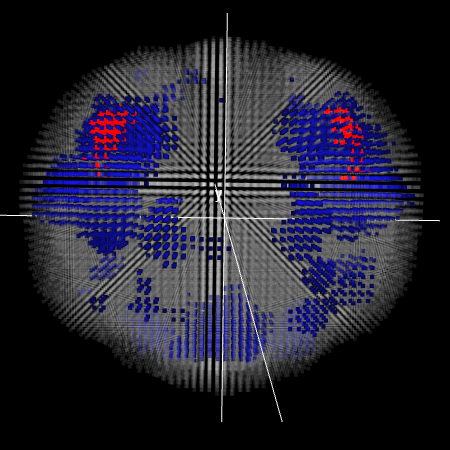
\includegraphics[width=.45\linewidth]{gfx/chapter2/cell4.png}}
        \caption{Regions defined by the expression overlap of the top 3 scoring genes in \cite{Tomer10} binarized in-situ hybridization data. The red colour shows the co-expression of the three considered genes, the blue areas are those where one or more of the three considrered genes are expressed but not all, in grey are the areas where none of the considered genes are expressed. The 4 figures are from a apical view with the dorsal side on top.}\label{fig:cell_localization}
\end{figure}

Overall, the results of this back-mapping method look very promising. Although at the time of writing, this work is still in progress in collaboration with Kaia Achim and Detlev Arendt, I have been able so far to map-back 27 of the 38 live single cells to a defined area of overlapping expression in the brain using the top 3 or 4 most specific genes. The cells were mapped to an average of 100 cubes defining a spatially coherent region. Interestingly later in this thesis, in Chapter \ref{ch:biology}, I find that the optimal number of clusters corresponding to potential cell types is 33 for the same dataset of 32.203 sites, which makes an average around 300 ``cubes'' per cell types, the same order of magnitude as the regions the single cells are mapped to.  \\

I decided to check the probability of obtaining such a result by chance. To this end, I randomly generated 1000 ``top 3'' genes out of the 86 genes considered in the in-situ hybridization data. For each of these ``top 3'' randomly generated genes, I computed the number of cubes in the in-situ hybridization dataset where the 3 genes were co-expressed.\\

Subsequently, I compared the number of overlapping cubes obtained with this random process to the number of overlapping cubes obtained with the top 3 most specific genes from the 38 live single cells. The results are shown as boxplots in Figure \ref{fig:boxplot_rna}. The left hand part of the plot shows the number of cubes obtained with the genes selected randomly. In this case the mean number of cubes if extremely close to zero . The right hand part of the plot shows the same results for the top 3 most specifically expressed genes of the 38 alive cells in the single cell RNA-seq dataset. A t test analysis of between the random and the RNA-seq observations yields : $pval = 0.0153$. In this context it is clear that the mapping result obtained is very likely to have some biological meaning.

	\begin{figure}[H]
\centerline{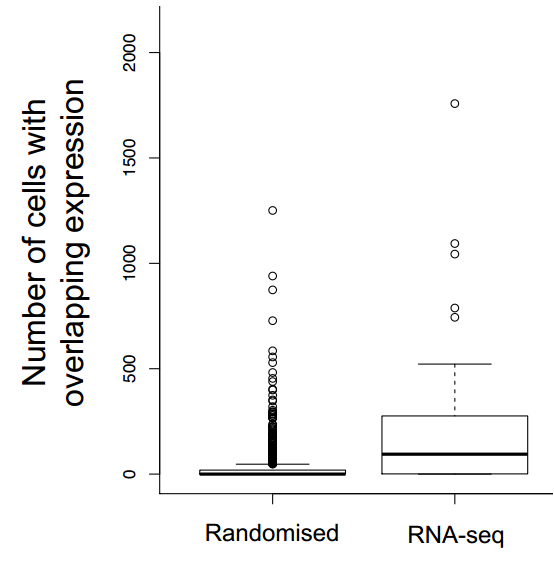
\includegraphics[width=0.6\linewidth]{gfx/chapter2/rand_top3.png}}
\caption{{\bf Back-mapping by chance vs RNA-seq data.} This boxplot shows the number of ``cubes'' in which the top 3 genes overlap with randomly generated top 3 genes (left N=1000) and the top 3 genes obtained from the live single cells RNA-seq data(N=38).}\label{fig:boxplot_rna}
	\end{figure}
	
  \subsection{Binarizing whole transcriptomes}
  
  Even though the back-mapping method describe previously manages to deal with the noise in the data by looking at the most specifically expressed genes, as mentioned for in-situ hybridization, for other methods it could be useful to binarize the data. When dealing with whole transcriptomes, manually finding thresholds to binarize gene expression data is no longer a valid option due to the high number of genes considered. An automated method is thus required. I will discuss possible ways to binarize single cell RNA-seq data, presenting some results cells from the brain of \platy{}.\\
  
  A naive approach would be to simply consider that as long as one RNA fragment mapped to a particular gene has been found in a cell, the gene is considered as expressed. Although such a method would be justifiable in the case of a perfect dataset, with no noise or errors, as discussed above \ref{sec:quantitative_single_cell} in the case of single cell RNA-seq the biases created by the mRNA capture rate are to high to rely simply on this method. Indeed, as a first approach on \platy{}'s dataset, we can see on Figure \ref{fig:hist_rna} that the value $0$ represents a very dominant peak. The problem in that case is that for read counts of $0$ it is dangerous to consider the gene as non expressed when it could be lowly expressed.\\
  
\begin{figure}[H]
        \myfloatalign
        \subfloat[Histogram showing the frequencies of count values over 72 sequenced cells, with the fragments mapped to 169 genes.]
        {\label{fig:hist_rna}
        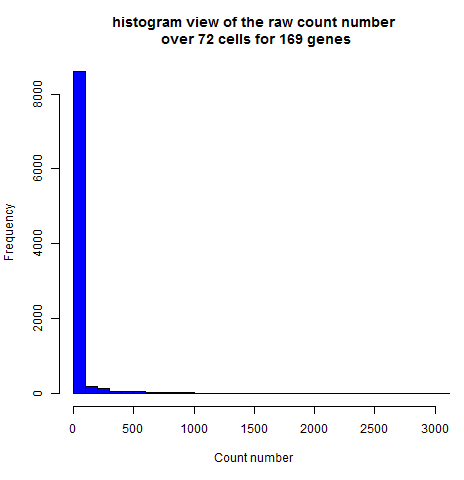
\includegraphics[width=.8\linewidth]{gfx/chapter2/hist_rna.png}} \\
        \subfloat[Density plot for the count values over $0$ in the single cell sequencing dataset]
        {\label{fig:density_rna}%
         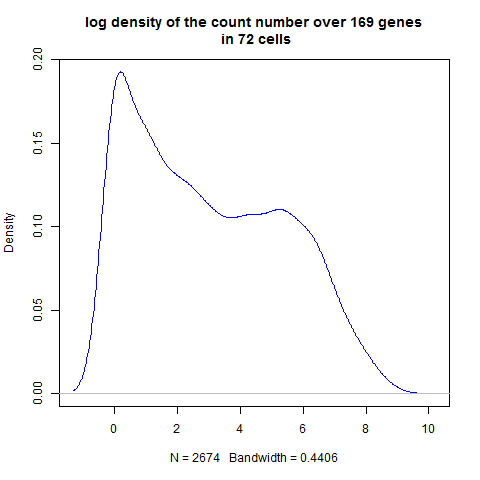
\includegraphics[width=.8\linewidth]{gfx/chapter2/density_rna.png}}
        \caption{Thresholding RNA sequencing data for \platy{}. The RNA-seq reads are mapped for the 72 cells to 169 genes in the PrimR dataset. This choice was made because at the moment the full genome of \platy{} is not available for mapping the reads. I believe however that mapping to the entire genome would improve the results significantly.}\label{fig:platynereis_single_cell}
\end{figure}
  
  Another option would be to find a global threshold over the complete dataset. The threshold, $T>0$, would represent the count number of reads for a particular gene and a particular cell needed to consider the gene as expressed. $T$ could be inferred from the count density over all the genes and all the cells. The expected result would be a 2 peak density with one peak corresponding to the non expressed count values, the second to expressed genes. The binary threshold would then be set between the first and second peak. Although more precise than the previous method, binarizing in such a manner may lead to numerous errors. Indeed, the underlying assumption behind this method is that all genes behave in a similar way. As Figure \ref{fig:density_rna} shows, if a 2 peak behaviour is indeed present, the cut is not extremely clear and an important portion of count numbers actually fall in between the two peaks. This is due to the fact that all expressed genes are not expressed in the same way; some are expressed lowly, some highly. As a result, the density curve tends to flatten making this thresholding method, if better, still not 100\% reliable.\\
  
  The more suitable approach to this thresholding problem would be to compute one threshold per gene based on the density curve for every gene across all cells. However, considering the sparse nature of the count data, no significant results can be extracted with this method without a large enough number of sequenced cells. However, I believe that one threshold per gene would result in a big improvement over the previously mentioned thresholding methods providing sufficient number of data points per gene.



\section{Conclusions}
In this Chapter I have described how the scale of gene expression studies has shifted from the tissue level to the single cell level. For two experimental protocols the generation of such data was presented and I have explained why, at the time of writing, it is still not safe to assume that single cell transcritomics datasets are quantitative. To avoid this problem, turning those datasets into binary gene expression is an attractive solution. However the binarization process is not trivial and I have presented ways to obtain a high confidence dataset.\\

One notable advantage of in-situ hybridization assays is the fact that the spatial information stays attached to each gene expression fingerprint. Using this information, it was possible to allocate cells assayed via single cell RNA-seq to their spatial location in the brain using the most specifically expressed genes in every cell. \\

As mentioned previously in the Introduction (\ref{ch:background}), if the ability to study the heterogeneity of cell populations at the single cell level offers incredible possibilities for the future of developmental biology and potentially of cancer research, the development of new statistical methods adapted to this single cell scale, allowing conclusions to be drawn at the tissue level, is crucial.\\

The work presented hereafter aims to answer simple but important questions: can known functional tissues of a complex organ like the brain be defined and localized from single gene expression data? Can unknown regions in such a complex tissue be detected and finally, is it possible to hypothesize the functional role of those unknown regions based on single cell expression data?


	
	



%*****************************************
%*****************************************
%*****************************************
%*****************************************
%*****************************************
%\addtocontents{toc}{\protect\clearpage} % <--- just debug stuff, ignore
%%************************************************
\chapter{Clustering tissues from single cell expression data and visualizing them in a 3D space}\label{ch:non_spatial_clustering_visualization} 
%************************************************
\section{Elements of clustering for biological tissues}
	\subsection{Why cluster?}
    - Single cell data has a lot of potential but:
    - Big data general problem
    - need to be able to come back from the single cell level to the tissue for : a consistency check and improve the knowleddge at the tissue level from single cell level

	\subsection{General considerations about clustering}
    - No perfect method
    - directed vs undirected
    - choosing the number of cluster, a key issue

\section{Visualizing clustering results in 3D with bioWeb3D}
	\subsection{Background}

Visualisation is a key feature in the analysis of large biological datasets, especially when analysing organized structures with distinct sub-clusters \cite{Rubel10}. This is particularly important when analysing 3-Dimensional (3D) datasets. When a biological process or feature has been described spatially by a set of 3D referenced points, either via laboratory work (confocal microscopy for example) or generated within a simulation, with some data attached to each point in space, the first step in interpreting the data is to visualise it. Once the data are visualised and the quality assessed, downstream analysis can proceed. For example, on obvious second step is to cluster the observations into different classes based upon the information assiciated with each point; those results will also need visualisation. \\

While various 3D visualisation tools have been developed, they have typically been made available via a locally installed piece of software such as BioLayout Express$^{3D}$\cite{Freeman07}, Arena3D \cite{Pavlopoulos08},  3D Genome Tuner \cite{Wang09}, the Allen Brain Atlas \cite{Lein07} or Cytoscape \cite{Shannon03}. Other 3D visualisation tools have been built online and are accessible through the browser directly, such as AstexViewer \cite{Hartshorn02}, which is utilised by the Protein Databank Europe via a Java Applet. More recently, visualisation tools developed using HTML5/WebGL capabilities have been described, although they have focused on very specific applications, such as analysing radiology data  \cite{Dinesh12}.\\
Importantly, as yet no tool has allowed biologists to view their own 3D data directly online in an easy, fast and interactive and secure way. Using webGL and the JavaScript 3D library Three.js, bioWeb3D aims to be a simple, generic, tool for tackling this problem.\\


	\subsection{Implementation}

bioWeb3D allows the user to represent any 3D dataset on their browser by defining only two files. The two files can either be formatted as JSON files, a widely used structured format on the web \cite{Wilde07} or directly as Comma Separated Values files (CSV).\\

The first file used by the application, referred to as the ``dataset file", contains the coordinates of every point in the dataset. The second type of file used, the ``information layer" file, describes one or several information layers that are associated with the points defined in the first file. For example, if each point defines the location of a cell within a tissue, the second file could describe whether a particular gene is expressed in each cell. That way the tissue expression profile can be represented in the spatial context of the tissue.\\

Datasets can be viewed and compared in up to four ``worlds" (each world refers to a separate visualisation sub-window) at the same time. Although browser based, the application, fully written in Javascript, does not need to send any data to the host server. Instead the modern internet browser's local file system reading capabilities are used through the HTML 5 FileReader functionality. This allows the application to handle, in a very short period of time, large datasets while ensuring that the privacy of the data is maintained.\\

Although the focus is on making bioWeb3D simple and easy to use, some options are available to customise how datasets are represented. The application can be used to visualise sequential information, such as 3D protein structures, in which case links can be drawn between the points. In other situations, such as when a population of cells is considered, the points can be left unlinked as individual particles. The information layers are visualised by colouring the 3D points according to the class that each point belongs to.

		\paragraph{technological overview}
bioWeb3D is fully written in HTML/Javascript. It relies heavily upon a relatively recent 3D javascript library called Three.js \cite{three}. This library is used as the main interface between webGL (cross-platform, royalty-free web standard for a low-level 3D graphics API) \cite{webgl}. More specifically, bioWeb3D allows the generation and manipulation of simple Three.js objects. Indeed the primary challenge associated with the creation of bioWeb3D has been to design interactions between the 3D visualisation and the user interface in the most efficient way.\\
		\paragraph{Defining the input files formats}
Using the JSON format to input files into bioWeb3D is recommended because of its rigorous structure, which allows fast Javascript object generation within the browser interpreter. Compared to other data-interchange languages, such as XML, JSON is also easily human readable thanks to a light-weight syntax. It is also supported by all of the primary internet browsers.\\
However, much data generated in the biological sciences is stored within CSV files. Converting CSV documents to the JSON format used in this application is not always trivial. In order to facilitate this process, the application is also able to interpret simple CSV files following a certain format as an input.


		\subsubsection{Dataset files specification}
When the user adds a new {\it{Dataset}} file, a new Dataset section is created in the ``Data" panel of the application. One raw data file contains one dataset.\\
		\paragraph{JSON format}
The {\it{dataset}} file should have a root object called ``dataset" which contains: \begin{itemize}
\item{The ``name" property of the dataset (\textit{e.g.}, ``my dataset");}
\item{The ``chain" parameter, which should be set to \textit{true} if the points are linked (the default value is \textit{false}) - the data will be considered sequentially, with each point linked according to its order in the dataset file;}
\item{The ``points" property, which is a two dimensional array representing a list of (x,y,z) vectors that define the co-ordinates of the points.}
\end{itemize}

Listing \ref{jsondataset} is an example of a minimal 3 points dataset file:

		\paragraph{CSV format}
Each line represents a point and the three coordinates on each line must be separated by ``comma" characters.\\As an example, listing \ref{csvdataset} carries the same information as the JSON file in Listing \ref{jsondataset}. Do note that although the spatial information remains the same it is not possible to set a name or to link the points within a CSV file input.



		\subsubsection{Information layer file specification}The {\it{Information layer}} file contains information about the points described in the Dataset file. The information in this file has to be given in the same order as the points defined in the Dataset file.

		\paragraph{JSON format}
The {\it{information layer}} files must have a root element named  ``information". Since one information file can define multiple information sets, the structure below ``information" is a list. Each element of the list is structured as follows:
\begin{itemize}
\item{The ``name" property (optional);}
\item{The ``numClass" property, which indicates the number of different classes the data will be assigned to;}
\item{The ``labels" property, which defines a list of names for the ``numClass" classes previously defined (optional);}
\item{The ``values" property, which defines the class of each point in the dataset. As points do not have single IDs, this property must be in the same order and have the same length as the points defined in the {\it{dataset}} file.}
\end{itemize}

For example coming back to the 3 points defined in Listing \ref{csvdataset} and Listing \ref{jsondataset}, two information layers could correspond to: 
\begin{itemize}

\item{one clustering algorithm that puts the first two points together in class one and the third point alone in a second class}
\item{a second clustering algorithm that puts each point in a separate class}
\end{itemize}

In this case the Information layer file would look like Listing \ref{jsoninfo}.


		\paragraph{CSV format}
Each column will represent in which class each point belongs. The separation character between columns must be a ``comma". Listing \ref{csvinfo} carries the same information as Listing \ref{jsoninfo}. Note that it is not possible to use the ``labels" or ``name" properties available in Listing \ref{jsoninfo} within a CSV information layer file. 




	\subsection{Results and Discussion}


		\paragraph{Basic usage}
	In figure 1 is visualised as an example, the brain the marine annelid {\it{Platynereis dumerilii}} each point represents a cell in the brain, the colour of which indicates the class it belongs to. The user can interact with the visualisation via an interface on the right of the screen, which contains three panels. In the ``dataset" panel, the user can choose the {\it{datasets}} and {\it{information layer}} files that should be represented in each world. This panel also allows the user to show/hide specific classes of the selected information layers. Each dataset file entered will create a new sub-panel where the user can input {\it{information layer}} files for that world. Selecting an {\it{information layer}} in the drop-down list will display the data in the current world and generate a list of classes that the user can modify regarding their visibility and colour. The ``View" panel enables the user to choose which of the worlds are shown on the screen, ranging from 1 to 4 simultaneous worlds. Finally, the ``Settings" panel provides the user with a number of options that affect all worlds and all datasets, such as modifying the axes scales.

		\paragraph{bioWeb3D and local software}
Many 3D visualisation software tools, most of which require local installation, exist and provide similar functionalities with standard 3D format input such as Wavefront .OBJ. Some are extremely generic and powerful like Blender. However, these tools are not typically oriented towards a scientific audience. Moreover, those that are more focused on science are often targeted towards a very specific application, especially in medical sciences \cite{Wang09}. In this context, we believe that bioWeb3D can be useful as it is completely generic and browser based. It should also be noted that recent browser improvements regarding GPU acceleration through the webGL paradigm allow bioWeb3D to visualise several hundred thousand points. Additionally, local software is usually platform specific, which is not the case for browser based applications.

		\paragraph{bioWeb3D and Java Applets}
As mentioned previously, browser based 3D visualisation tools currently exist mainly in the form of Java Applets. This technology has attracted much criticism in 2012 regarding security flaws, leading the ``United States Computer Emergency Readiness Team" to advise that all Java Applets should be disabled due to current and future Java vulnerabilities \cite{security}. The development of WebGL technology is viewed by many as a candidate for replacing Applets. 



		\paragraph{Current limitations}
The main current limitation of a webGL based application is the machine and browser compatibility. Only computers with fairly recent graphic cards will be able to run a 3D environment. It should also be noted that Microsoft has notified the developer community that Internet Explorer is not scheduled to support WebGL in the near future. However, importantly, Chrome, Firefox, Safari and Opera all now support webGL applications. It could also be important to mention for eventual future developments that webGL is supported on mobile platforms such as iOS or Android. \cite{caniuse}

	\subsection{Conclusions}
bioWeb3D is designed to be a simple and quick way to view 3D data with a specific focus on biological applications.  Being browser-based, the software can be easily used from any computer without the need to install a piece of software. Importantly bioWeb3D has been designed to offer a very straightforward and easy-to-use working environment. Despite the current limitations in terms of compatibility or rendering performances for large numbers of points, we believe that bioWeb3D will enable non-experts in 3D data representation to quickly visualise their data and the information attached to it in many biological context, thus facilitating downstream analyses.

	\subsection{Availability and requirements}
The full source code is available on the github page of the project \cite{github}. A live version of the software is online \cite{bioWeb3D}. You will require a graphical card and a browser with webGL capabilities to run bioWeb3D.

\section{Non spatial clustering methods}
	\subsection{Hierarchical clustering}
    - General description of the method
    - Computing distance matrix on binary expression data
    - Hclust method to use (full or partial)
    - Discuss the choosing the K with hClust (dendrogram is not informative)
 
	\subsection{Independent mixture models}
    - General statistical framework
    - Present the model
    - Gene independence hypothesis (this will be discussed further in the next chapter)
    - Likelihood of the model
    - EM algorithm to maximize the parameters (theta)
    - Choosing K with the BIC

\section{Discussion}
	\subsection{Spatial clustering techniques (hierarchical, model based)}
    - Limits of non spatial methods on noisy data (cite the "cell model of chapter 1" paragraph)
    - Not using the spatial data seems silly when we do have it (playing chess blind comparison ?)
    - Some clustering methods are able to take into account the spatial localization of the data points as well as the expression data
    - Quickly present spatial methods (spatial hclust), Mixture with a spatial component

	\subsection{Method chosen}
    - MRF because theta parameters are informative, easy to compute a likelihood and to choose K




%*****************************************
%*****************************************
%*****************************************
%*****************************************
%*****************************************

%\include{multiToC} % <--- just debug stuff, ignore for your documents
% ********************************************************************
% Backmatter
%*******************************************************
\appendix
\cleardoublepage
\part{Appendix}
%********************************************************************
% Appendix
%*******************************************************
% If problems with the headers: get headings in appendix etc. right
%\markboth{\spacedlowsmallcaps{Appendix}}{\spacedlowsmallcaps{Appendix}}
\chapter{Full list of the clusters obtained with the HMRF method}
This chapter provides a quick glance over the 33 clusters generated by the HMRF method (see Chapters, \ref{ch:HMRF} and \ref{ch:biology}) in the brain of \platy{} using the $86$ genes selected from the in-situ hybridization data generated by Raju Tomer. Each cluster is presented from an apical point of view alongside the adult eyes (red cluster) for spatial reference. On each images the 3 top scoring (see Chapter \ref{ch:biology} for an explanation of the scoring process) genes are indicated.\\

\renewcommand{\thesubfigure}{\roman{subfigure}}

\begin{figure}[bth]
        \myfloatalign
        \subfloat[Cluster 1]
        {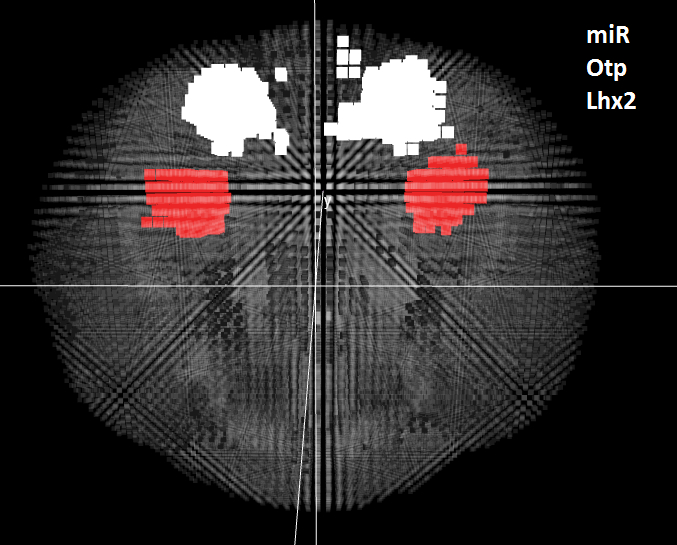
\includegraphics[width=.45\linewidth]{gfx/sup/c1.png}} \quad
        \subfloat[Cluster 2]
        {
         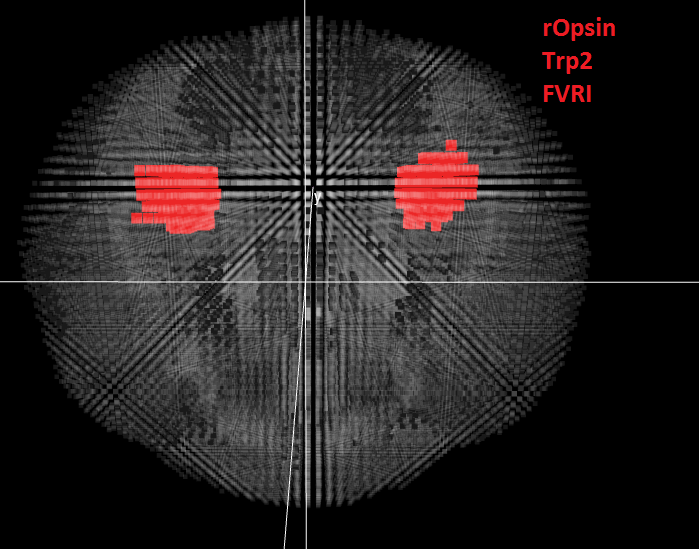
\includegraphics[width=.45\linewidth]{gfx/sup/c2.png}} \\
        \subfloat[Cluster 3]
        {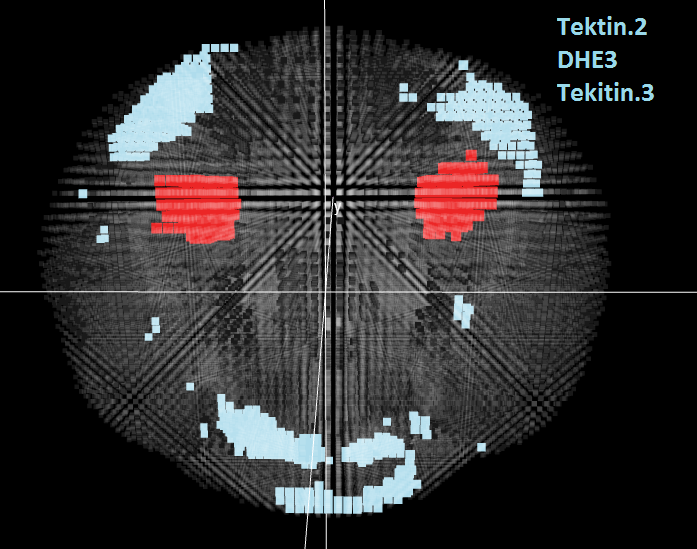
\includegraphics[width=.45\linewidth]{gfx/sup/c3.png}} \quad
        \subfloat[Cluster 4]
        {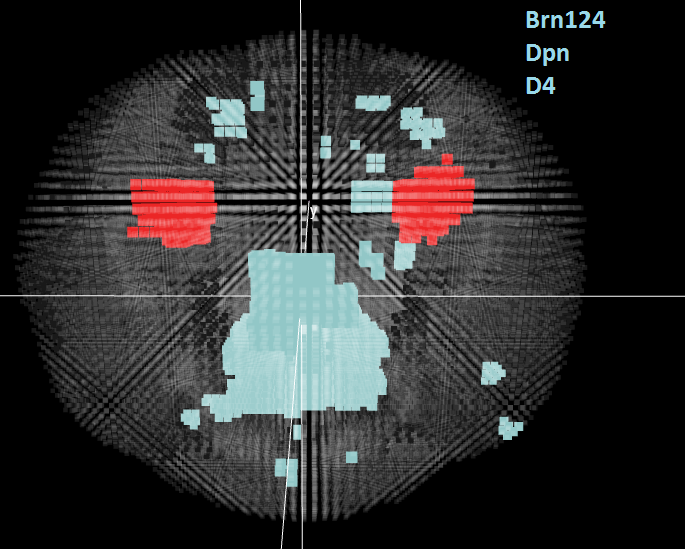
\includegraphics[width=.45\linewidth]{gfx/sup/c4.png}} \\
        \subfloat[Cluster 5]
        {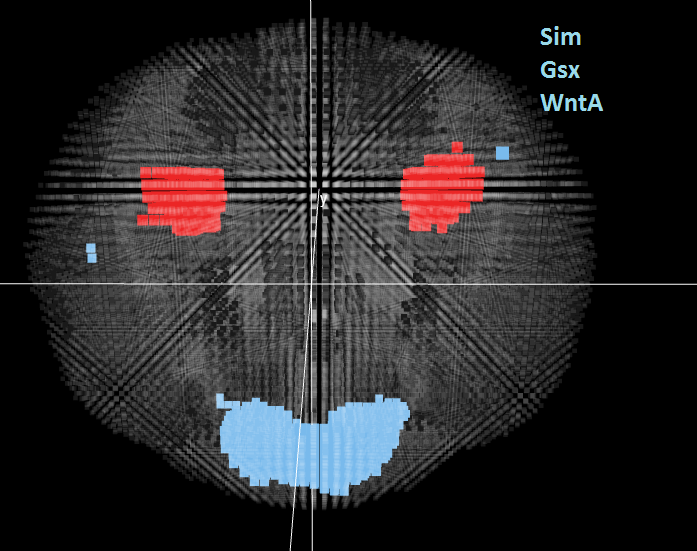
\includegraphics[width=.45\linewidth]{gfx/sup/c5.png}} \quad
        \subfloat[Cluster 6]
        {
        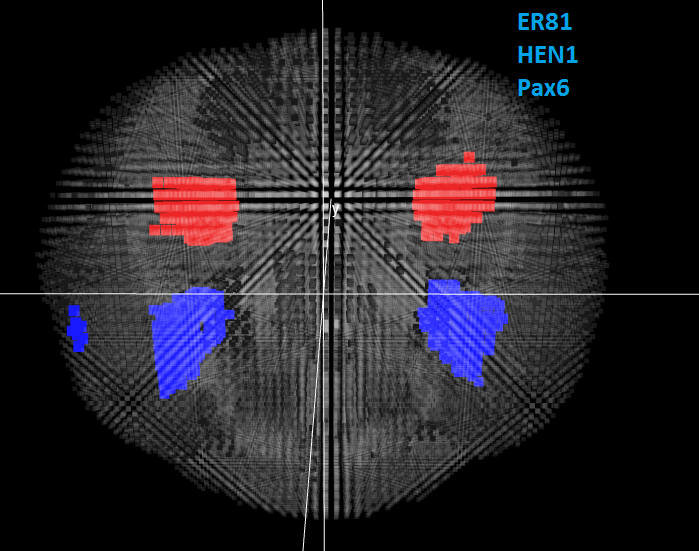
\includegraphics[width=.45\linewidth]{gfx/sup/c6.png}} \\
        \subfloat[Cluster 7]
        {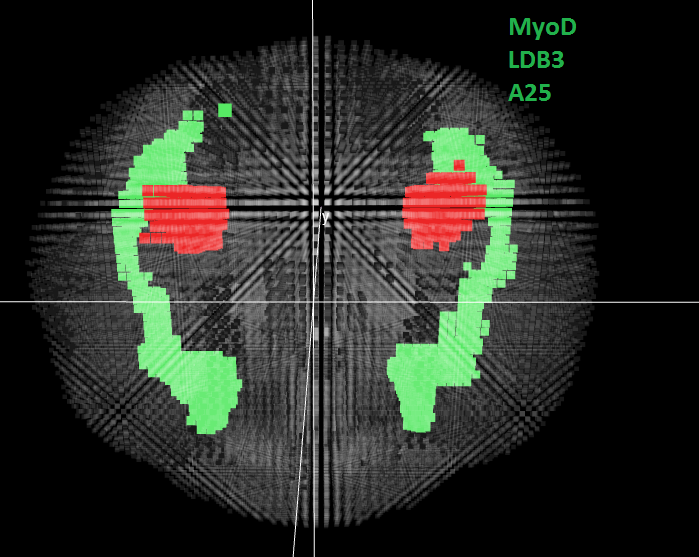
\includegraphics[width=.45\linewidth]{gfx/sup/c7.png}} \quad
        \subfloat[Cluster 8]
        {
        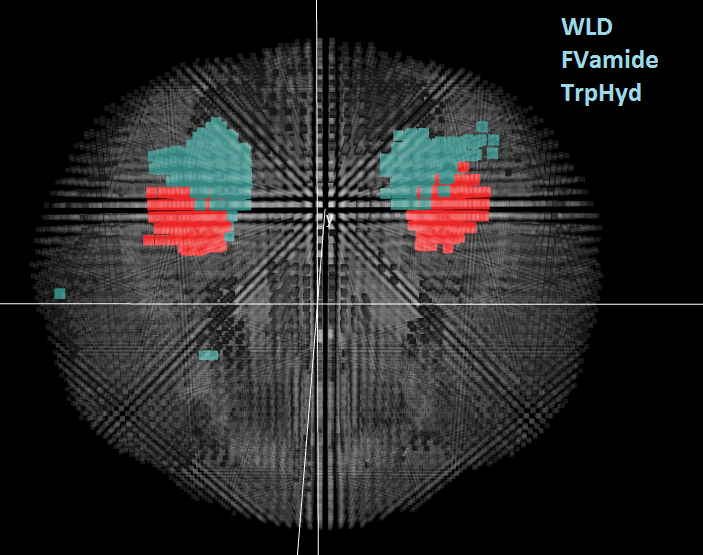
\includegraphics[width=.45\linewidth]{gfx/sup/c8.png}} \\
        \subfloat[Cluster 9]
        {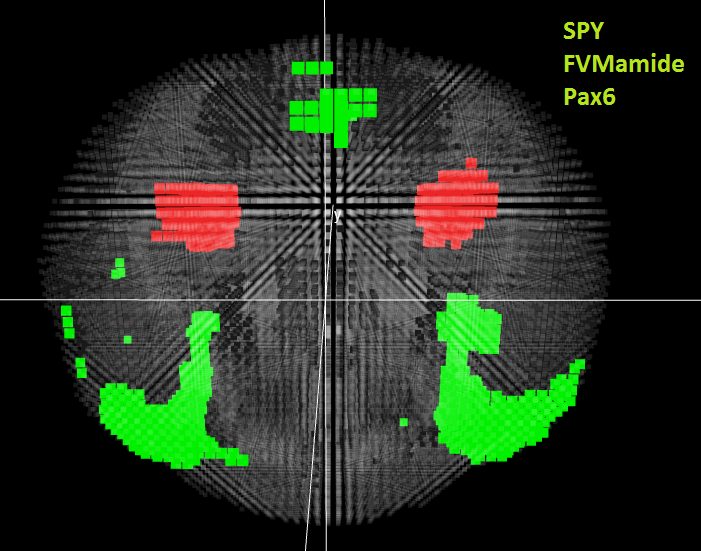
\includegraphics[width=.45\linewidth]{gfx/sup/c9.png}} \quad
        \subfloat[Cluster 10]
        {
        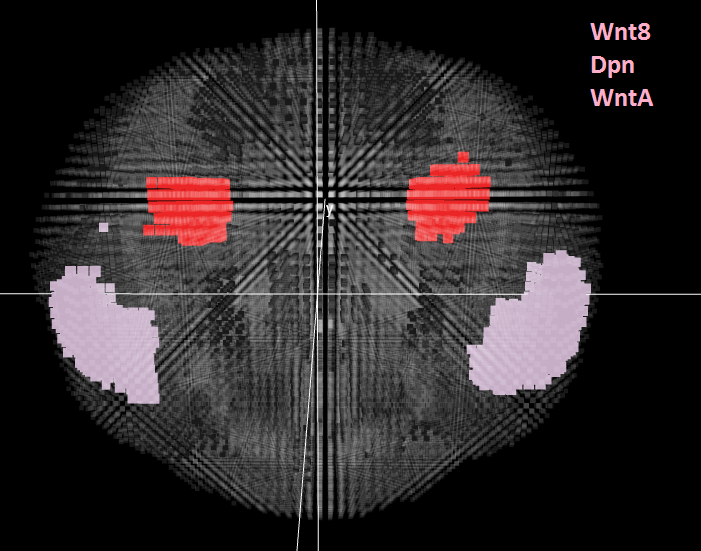
\includegraphics[width=.45\linewidth]{gfx/sup/c10.png}}
\end{figure}

\begin{figure}[bth]
         \ContinuedFloat 
        \subfloat[Cluster 11]
        {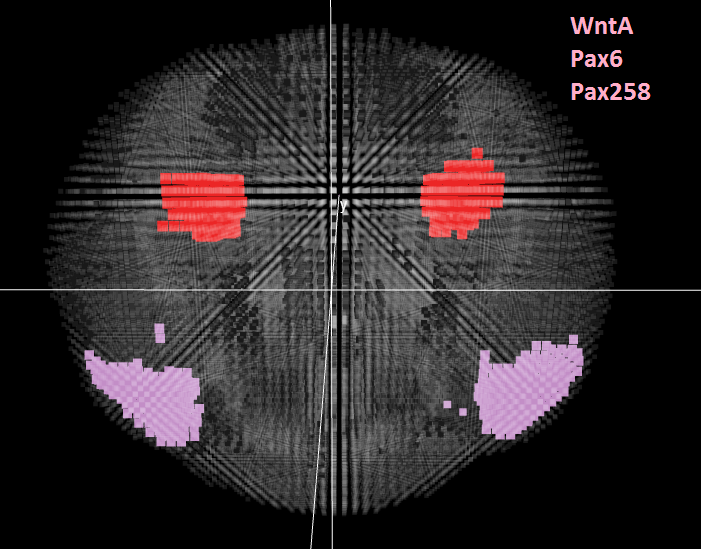
\includegraphics[width=.45\linewidth]{gfx/sup/c11.png}} \quad
        \subfloat[Cluster 12]
        {
        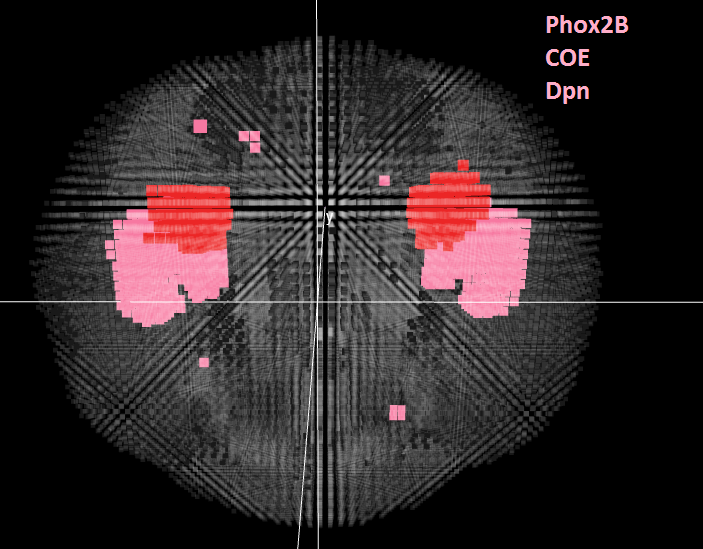
\includegraphics[width=.45\linewidth]{gfx/sup/c12.png}} \\
        \subfloat[Cluster 13]
        {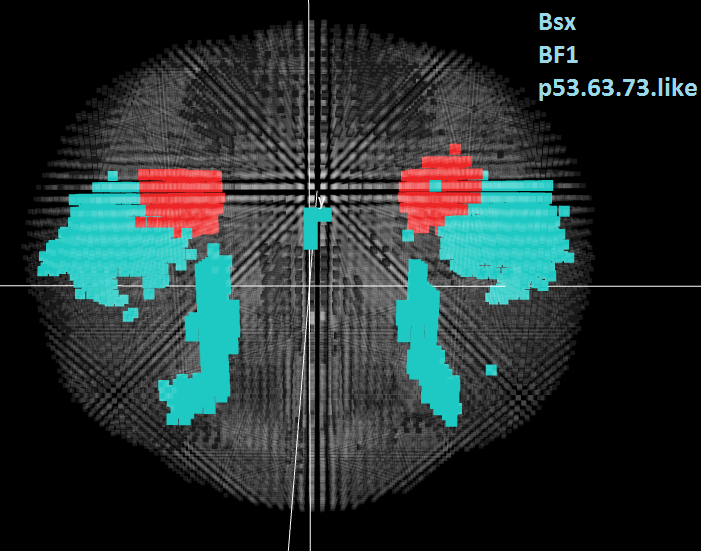
\includegraphics[width=.45\linewidth]{gfx/sup/c13.png}} \quad
        \subfloat[Cluster 14]
        {
        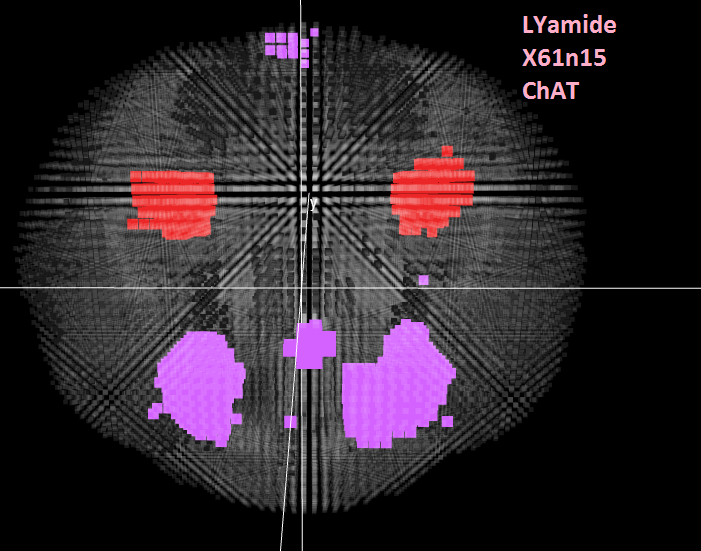
\includegraphics[width=.45\linewidth]{gfx/sup/c14.png}} \\
        \subfloat[Cluster 15]
        {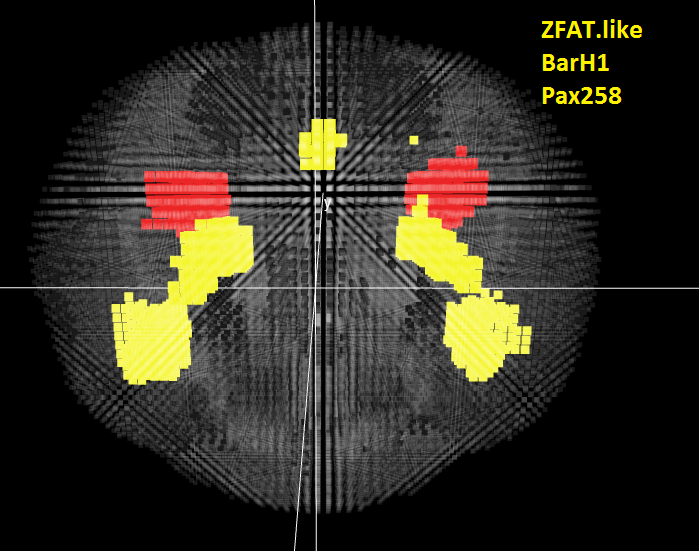
\includegraphics[width=.45\linewidth]{gfx/sup/c15.png}} \quad
        \subfloat[Cluster 16]
        {
        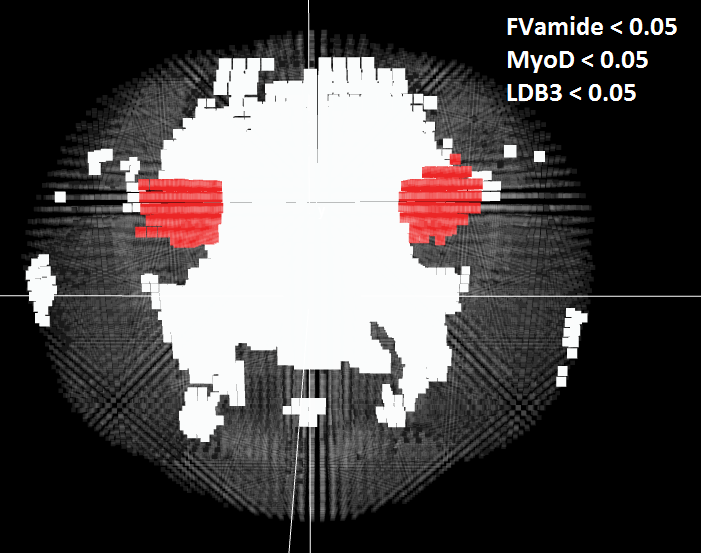
\includegraphics[width=.45\linewidth]{gfx/sup/c16.png}} \\
        \subfloat[Cluster 17]
        {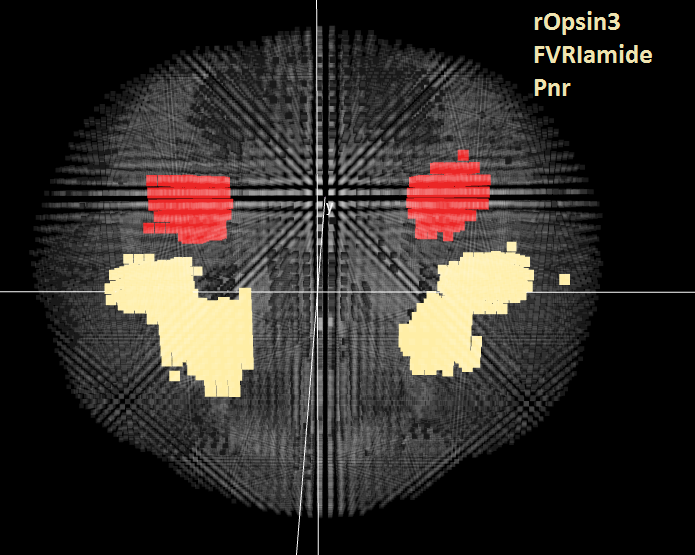
\includegraphics[width=.45\linewidth]{gfx/sup/c17.png}} \quad
        \subfloat[Cluster 18]
        {
        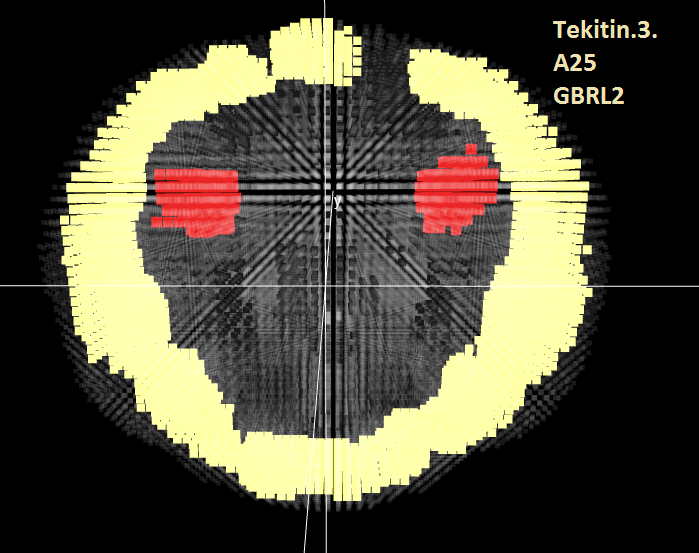
\includegraphics[width=.45\linewidth]{gfx/sup/c18.png}} \\
        \subfloat[Cluster 19]
        {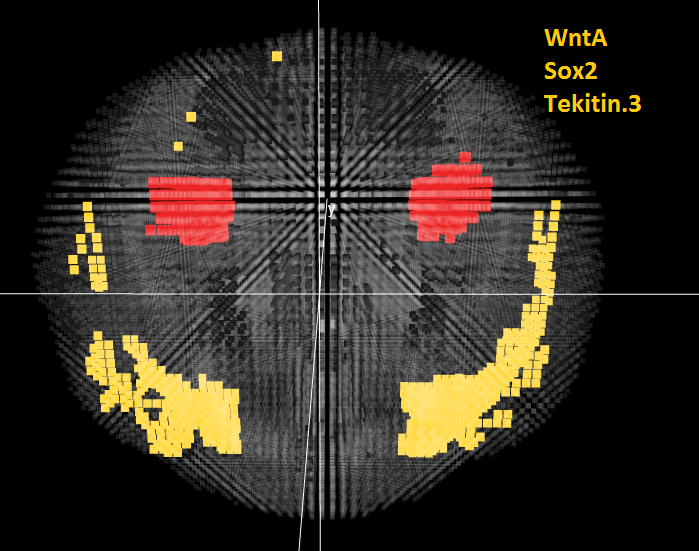
\includegraphics[width=.45\linewidth]{gfx/sup/c19.png}} \quad
        \subfloat[Cluster 20]
        {
        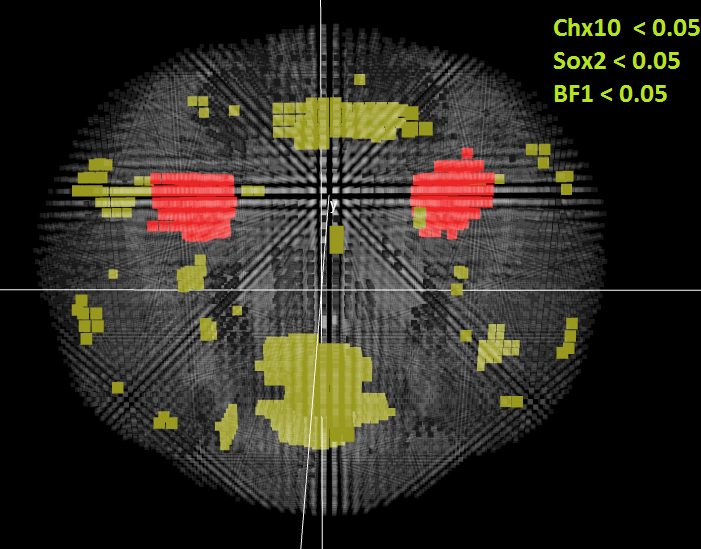
\includegraphics[width=.45\linewidth]{gfx/sup/c20.png}}
\end{figure}

\begin{figure}[bth]
       \ContinuedFloat 
        \subfloat[Cluster 21]
        {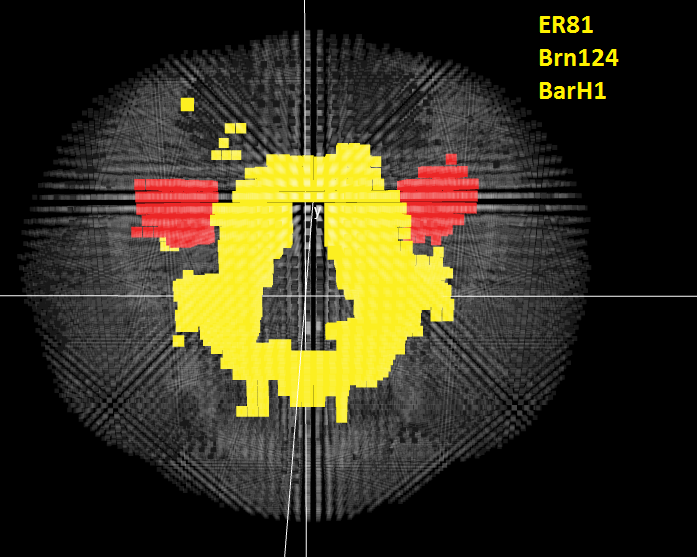
\includegraphics[width=.45\linewidth]{gfx/sup/c21.png}} \quad
        \subfloat[Cluster 22]
        {
        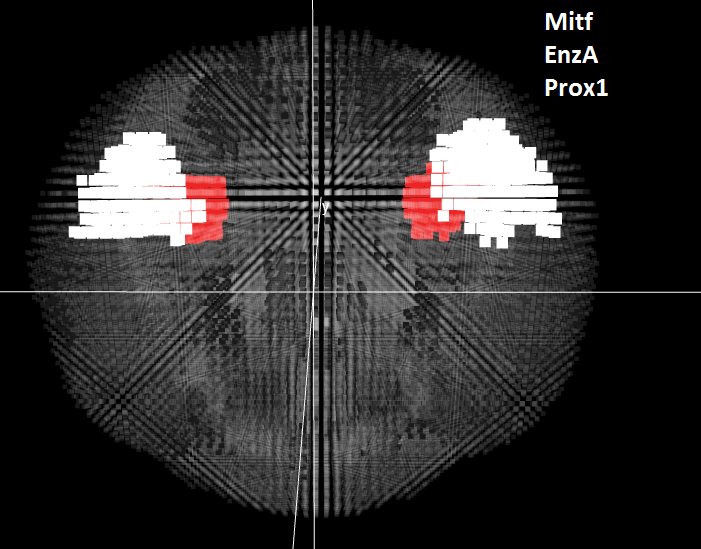
\includegraphics[width=.45\linewidth]{gfx/sup/c22.png}} \\
        \subfloat[Cluster 23]
        {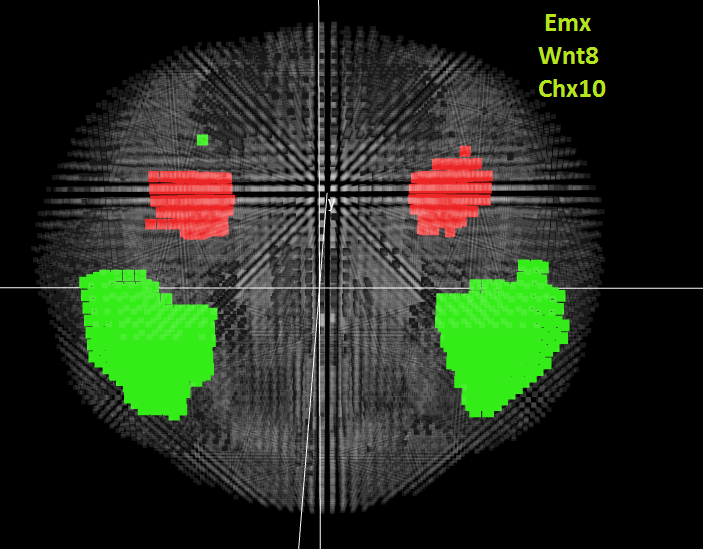
\includegraphics[width=.45\linewidth]{gfx/sup/c23.png}} \quad
        \subfloat[Cluster 24]
        {
        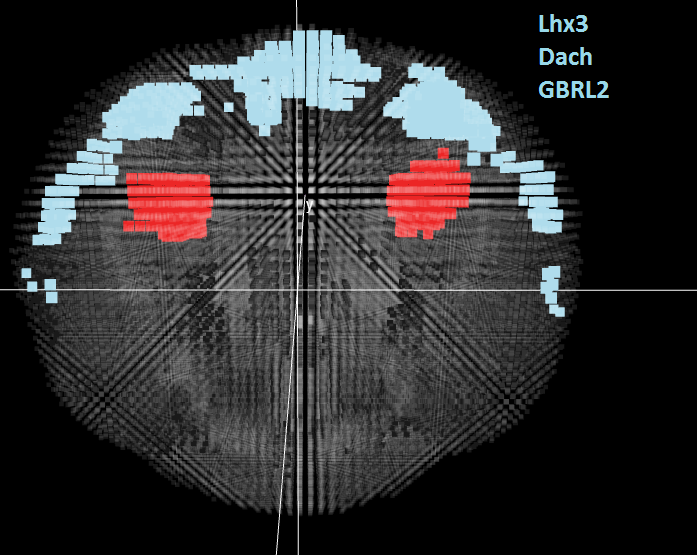
\includegraphics[width=.45\linewidth]{gfx/sup/c24.png}} \\
        \subfloat[Cluster 25]
        {\includegraphics[width=.45\linewidth]{gfx/sup/c25.png}} \quad
        \subfloat[Cluster 26]
        {
        \includegraphics[width=.45\linewidth]{gfx/sup/c26.png}} \\
        \subfloat[Cluster 27]
        {\includegraphics[width=.45\linewidth]{gfx/sup/c27.png}} \quad
        \subfloat[Cluster 28]
        {
        \includegraphics[width=.45\linewidth]{gfx/sup/c28.png}} \\
        \subfloat[Cluster 29]
        {\includegraphics[width=.45\linewidth]{gfx/sup/c29.png}} \quad
        \subfloat[Cluster 30]
        {
        \includegraphics[width=.45\linewidth]{gfx/sup/c30.png}}
\end{figure}

\begin{figure}[bth]
       \ContinuedFloat
        \subfloat[Cluster 31]
        {\includegraphics[width=.45\linewidth]{gfx/sup/c31.png}} \quad
        \subfloat[Cluster 32]
        {
        \includegraphics[width=.45\linewidth]{gfx/sup/c32.png}} \\
        \subfloat[Cluster 33]
        {\includegraphics[width=.45\linewidth]{gfx/sup/c33.png}} \quad
        
        
         
        \caption{33 clusters generated by the HMRF method}\label{fig:clusters}
\end{figure}

%********************************************************************
% Other Stuff in the Back
%*******************************************************
\cleardoublepage%********************************************************************
% Bibliography
%*******************************************************
% work-around to have small caps also here in the headline
\manualmark
\markboth{\spacedlowsmallcaps{\bibname}}{\spacedlowsmallcaps{\bibname}} % work-around to have small caps also
%\phantomsection 
\refstepcounter{dummy}
\addtocontents{toc}{\protect\vspace{\beforebibskip}} % to have the bib a bit from the rest in the toc
\addcontentsline{toc}{chapter}{\tocEntry{\bibname}}
\label{app:bibliography} 
\bibliography{Bibliography}
\cleardoublepage\pagestyle{empty}

\hfill

\vfill


\pdfbookmark[0]{Colophon}{colophon}
\section*{Colophon}
This document was typeset using the typographical look-and-feel \texttt{classicthesis} developed by Andr\'e Miede. 
The style was inspired by Robert Bringhurst's seminal book on typography ``\emph{The Elements of Typographic Style}''. 
\texttt{classicthesis} is available for both \LaTeX\ and \mLyX: 
\begin{center}
\url{http://code.google.com/p/classicthesis/}
\end{center}
Happy users of \texttt{classicthesis} usually send a real postcard to the author, a collection of postcards received so far is featured here: 
\begin{center}
\url{http://postcards.miede.de/}
\end{center}
 
\bigskip

\noindent\finalVersionString

%Hermann Zapf's \emph{Palatino} and \emph{Euler} type faces (Type~1 PostScript fonts \emph{URW
%Palladio L} and \emph{FPL}) are used. The ``typewriter'' text is typeset in \emph{Bera Mono}, 
%originally developed by Bitstream, Inc. as ``Bitstream Vera''. (Type~1 PostScript fonts were made 
%available by Malte Rosenau and
%Ulrich Dirr.)

%\paragraph{note:} The custom size of the textblock was calculated
%using the directions given by Mr. Bringhurst (pages 26--29 and
%175/176). 10~pt Palatino needs  133.21~pt for the string
%``abcdefghijklmnopqrstuvwxyz''. This yields a good line length between
%24--26~pc (288--312~pt). Using a ``\emph{double square textblock}''
%with a 1:2 ratio this results in a textblock of 312:624~pt (which
%includes the headline in this design). A good alternative would be the
%``\emph{golden section textblock}'' with a ratio of 1:1.62, here
%312:505.44~pt. For comparison, \texttt{DIV9} of the \texttt{typearea}
%package results in a line length of 389~pt (32.4~pc), which is by far
%too long. However, this information will only be of interest for
%hardcore pseudo-typographers like me.%
%
%To make your own calculations, use the following commands and look up
%the corresponding lengths in the book:
%\begin{verbatim}
%    \settowidth{\abcd}{abcdefghijklmnopqrstuvwxyz}
%    \the\abcd\ % prints the value of the length
%\end{verbatim}
%Please see the file \texttt{classicthesis.sty} for some precalculated 
%values for Palatino and Minion.
%
%    \settowidth{\abcd}{abcdefghijklmnopqrstuvwxyz}
%    \the\abcd\ % prints the value of the length





\cleardoublepage%*******************************************************
% Declaration
%*******************************************************
\refstepcounter{dummy}
\pdfbookmark[0]{Declaration}{declaration}
\chapter*{Declaration}
\thispagestyle{empty}
This thesis:
\begin{itemize}
\item is my own work and contains nothing which is the outcome of work done in collaboration with others, except where specied in the text;
\item is not substantially the same as any that I have submitted for a degree or diploma or other qualication at any other university; and
\item does not exceed the prescribed limit of 60,000 words.
\end{itemize}
\bigskip
 
\noindent\textit{\myLocation, \myTime}

\smallskip

\begin{flushright}
    \begin{tabular}{m{5cm}}
        \\ \hline
        \centering\myName \\
    \end{tabular}
\end{flushright}

% ********************************************************************
% Game Over: Restore, Restart, or Quit?
%*******************************************************
\end{document}
% ********************************************************************
